\documentclass[12pt,a4paper,oneside]{book}

%\usepackage[Glenn]{fncychap}%format des titres des chapitres
% \usepackage[utf8]{inputenc} 


\usepackage[frenchb]{babel}
\usepackage[utf8]{inputenc}
\usepackage[T1]{fontenc}
\usepackage{amsfonts}
\usepackage{amsmath}
\usepackage{amsthm}
\usepackage{amssymb}
\usepackage{verbatim}
\usepackage{titlesec}
\usepackage{graphicx}
\usepackage{float}
\pagestyle{plain}
\usepackage{wallpaper}
\usepackage{mathtools}
\usepackage{tabularx}


\usepackage[linesnumbered,ruled,vlined]{algorithm2e}
\usepackage{algpseudocode}
\usepackage{apacite}

\usepackage[top=2.5cm, bottom=2.5cm, left=2.5cm, right=2.5cm]{geometry}
\theoremstyle{definition}
\newtheorem{definition}{Définition}[section]

\newcommand{\R}{\mathbb{R}}
\newcommand{\N}{\mathbb{N}}
\newcommand{\Z}{\mathbb{Z}}

\DeclarePairedDelimiter\ceil{\lceil}{\rceil}
\DeclarePairedDelimiter\floor{\lfloor}{\rfloor}
\DeclareMathOperator*{\mini}{min}



\begin{document}

    \begin{titlepage}

\newgeometry{top=0mm,right=20mm,left=20mm,bottom=0mm}



	%--------------------  Entete de l'Ecole ----------------------%

	\begin{figure}[t]
		
\includegraphics[scale=0.75]{ESI.png}\\[0.6in]
	\end{figure}
	
	
	
	%--------------------------------------------------------------%
	\begin{center}
	
	%------------------------  Le sujet ---------------------------%
		\LARGE \textbf{ Mémoire}\\
		\Large{
			Pour Obtention du diplôme de Master En Informatique\\
			\textbf{Option : Système Informatique (SIQ)}
			%\textsc thèse D'Ingéniorat En Informatique sous le thème :
		}\\
		\huge {
		\rule{\linewidth}{.5pt}
			\textbf{
				Méthodes d’optimisation hybrides : les heuristiques au service des méthodes exactes
			} 
			\rule{\linewidth}{.5pt}
		}\\[0.4in]
		\Large
	%--------------------------------------------------------------%	
	
	%-------------------------  Mon nom ---------------------------%
	\textbf{Réaliser par:}\\
	\begin{multicols}{}
			\Large 	Ali YADDADEN\\
			\large ea\_yaddaden@esi.dz\\
			ESI\\
		
	\end{multicols} 
	
	\vskip 0.13in
	%--------------------------------------------------------------%	

	%-----------------------  Encadreures -------------------------%
	 \textbf{Encadreur:}
	 
	 \begin{multicols}{}
			\Large 	Mme. Fatima BENBOUZID SI TAYEB\\
 			%\Large  M. Aziz MOUKRIM\\
 			%\Large  M. Jean\-Paul BOUFFLET\\
	\end{multicols}
	
	%--------------------------------------------------------------%	
	
	\small
	\vskip 0.5in
	Octobre 2018 \\
	Année Universitaire: 2018-2019\\
	
	\end{center}		
\restoregeometry
\end{titlepage}

    \listofalgorithms
    \listoffigures
    \tableofcontents
    \newpage
    \chapter*{Introduction générale}
    % Ce qui motive l'étude derrière les chapitres produits
    Les travaux en optimisation combinatoire touchent plusieurs axes de recherches tels que la programmation linéaire et non-linéaire, les méthodes reposants sur la génération de coupes ou de colonnes, les heuristiques, les métaheuristiques, les méthodes hybrides, etc. Ceux-ci trouvent beaucoup d'applications dans divers problèmes tels que l'ordonnancement, la planification, les problèmes logistique, la gestion de stock, etc. Au fil du temps et des divers travaux menés, divers idées ont émergées et touchent plusieurs aspects des méthodes d'optimisation et ceci dans le but de les rendre soit plus rapide ou bien plus précise et idéalement, les deux à la fois.
    
    L'une des approches qui a donné le plus de succès, est l'hybridation de méthodes exactes avec des heuristiques. Une revue de cette hybridation peut être a été faire par \cite{Puchinger2005}. Cela permet de profiter des avantages des deux. D'un côté les méthodes exactes garantissent des solution de très bonnes qualité et de l'autre, les heuristiques garantissent la rapidité d'exécution. Souvent, les problème auxquels on a affaire ont une formulation mathématique. On peut alors être amené à profiter des travaux fait sur le programmation linéaire et les adapter au problème. Les heuristiques primitives constituent une part fondamentale de la programmation linéaire et constitue l'un des principaux schémas d'hybridation entre méthodes exactes et heuristiques. Le schéma de parcours étant, le plus souvent dans ce cas, une méthode exacte arborescente dans laquelle est appelée une de ces heuristiques primitives.
    
    Dans cette optique, il serait intéressant d'aborder les méthodes exactes arborescentes existantes pour la résolution de problèmes d'optimisation et progressivement de voir les heuristiques primitives et quelques aspects de la programmation linéaires. Il serait aussi pertinent, dans la suite, de montrer la relation entre les heuristiques primitives et les méthodes exactes et quelques cas d'utilisation concrets en dehors des programmes linéaires abstraits. Il est à souligner que les contraintes modélisant un aspect du problème qu'on cherche à optimiser  rendent la résolution plus difficile, d'où l'intérêt de se pencher sur ce cas. 
    
    Dans ce mémoire, tous les aspects précédents seront abordés avec un premier chapitre sur les méthodes exactes arborescentes de résolution de problèmes d'optimisation. Dans le deuxième chapitre, on verra les heuristiques primitives. On verra aussi comment elles simulent un arbre branch-and-bound et comment elle s'incorporent bien dans les méthodes arborescentes. Dasn le dernier chapitre, on fera une sythèse de travaux dans lesquels les heuristiques primitives ont été utilisées pour résoudre des problèmes d'optimisation. Ceci permettra de confirmer ou d'infirmer l'utilité de celles-ci dans le processus de résolution. 

    %le fait d'avoir une formulation mathématique + efficacité travaux MIP ---> 	emploi sur des pbs --> heuristiques primitives
	\chapter{Méthodes exactes de résolution}
	\section{Introduction}
	La résolution de problème d'optimisation combinatoire nécessite souvent l'utilisation d'algorithmes très sophistiqués. Souvent, ces problèmes sont NP-difficile et il n'existe pas d'algorithmes polynomiaux pour leur résolution. C'est la cas par exemple du problème de sac à dos, de voyageur du commerce, de coloration de graphe, de tournée de véhicules, etc. pour lesquels une exploration exhaustive de l'espace de recherche n'est pas fructueuse. Cela nécessite donc faire une exploration intelligente de l'espace de recherche et par delà même, un choix de stratégies et de paradigmes de recherches suivant le but à atteindre. On peut donc vouloir la meilleure solution pour le problème et donc se référer aux méthodes dites \textit{"exactes"} ou bien une solution de bonne qualité et opter pour les méthodes dites \textit{"approchées"}. L'avantage des méthodes exactes est qu'elles trouvent la meilleure solution au problème mais cela au détriment d'un temps de calcul plus important. Elles sont donc privilégiées pour les petites instances. Les méthodes approchées donnent, quant à elles, une solution approximatives du problèmes tout en respectant certains critères de qualité pour la solution trouvée. Elles sont privilégiées quand le temps de calcul est borné et qu'une solution de bonne qualité seulement est suffisant. Notons aussi la combinaison des méthodes exactes et approchée est aussi un paradigme pour trouver de meilleures solutions approchées. Une revue des combinaisons de méthodes exactes et approchées peut être trouvée dans \cite{Puchinger2005}. 
	\paragraph{}
	Dans la suite, nous nous intéressons aux méthodes exactes de résolution de problèmes d'optimisation combinatoire et particulièrement aux méthodes d'exploration arborescentes de l'espace de recherche. 
	%conclure avec une bref enumération des méthodes qu'on va aborder.
	La reste de ce chapitre est organisé comme suit. D'abord on donnera une description du branch-and-bound et l'esquisse de l'algorithme. Les principales phases de l'algorithme seront elles aussi abordées. Ensuite, c'est le branch-and-cut qui sera abordé. On verra comment il diffère du branch-and-bound classique et quels choix sont cruciaux à faire dans cet algorithme. Enfin, la dernière variante est abordée. Il s'agit du branch-and-price. On verra aussi dans ce cas sur quel méthodes il repose et quels sont les choix qu'il incombe de faire au moment de sa conception. Dans les trois cas, quelques cas d'utilisation sont cités pour donner une idée de l'étendue de l'application de ces algorithmes.
	 
	\section{Branch and bound} \label{bb}
	\subsection{Description la méthode}
	%ici donner aussi des généralités sur les méthodes arborescentes
	La méthode de Branch and bound est une des méthodes les plus classiques et les plus répondues parmi les méthodes de résolution exactes. Elle fut introduit pour la première fois par \cite{Land1960}. Le principe est de faire une exploration intelligente de l'espace de recherche en éliminant implicitement une partie dont on sait à l'avance qu'elle ne contient pas une meilleure solution que celle actuellement trouvée. Ceci se fait par le calcul de bornes (suivant que cela soit un problème de maximisation ou de minimisation cela peut être le calcul d'une borne inférieure ou supérieure). Si l'on considère un problème de minimisation tel que le problème du voyageur du commerce, une solution actuelle trouvée $X$ constitue une borne supérieure. Donc toute solution $X'$ trouvée telle que \{ $f(X') \textgreater f(X)$, $f$ étant la fonction objectif \} est rejetée et l'espace de recherche lui correspondant est éliminé. C'est cette distinction des espaces de recherche qui fait que l'exploration est arborescente. A l'état initial, un seul espace de recherche existe, c'est l'espace des solutions au complet qui représente la racine des l'arbre et la borne est initialisée à $\infty$. A chaque itération, l'espace est partitionné en sous-espaces de recherche qui représentent les nœuds de l'arbre. Il s'en suit après trois principales procédures:
	\begin{enumerate}
		\item Sélection du prochain nœud à traiter
		\item Calcul des bornes
		\item Branchement (partitionner l'espace de recherche en sous-espaces de recherche)
	\end{enumerate} 
	Les étapes peuvent êtres représentés schématiquement comme sur l'illustration ci-dessous.
	%image du B&B
	\begin{figure}[H]
		\centering
		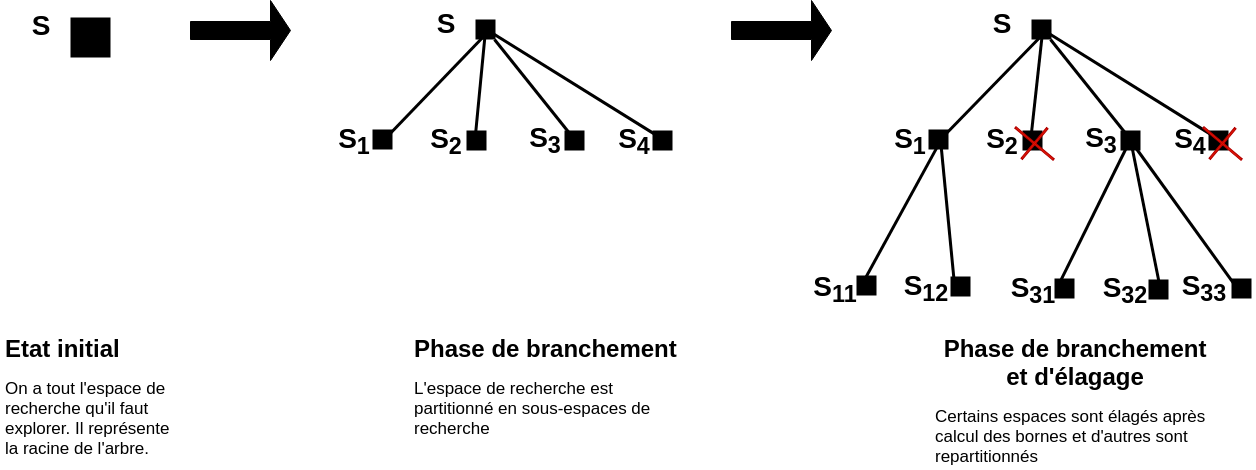
\includegraphics[width=0.9\linewidth]{schema_b&b}
		\caption{Schéma représentant les phases du Branch and bound}
		\label{fig:schemabb}
	\end{figure}
	
	Le séquencement des procédures citées ci-dessus peut varier selon la stratégie de sélection du nœud à traiter. Si le choix du prochain sous-problème se fait en fonction de sa borne, alors l'opération qui suit le choix du nœud est le branchement. L'espace des solutions est alors divisé en deux ou plusieurs sous-espaces. Si le sous-espace ne contient qu'une seule solution, sa valeur est alors calculée et comparée à la meilleure solution trouvée jusque-là. La meilleure des deux est alors gardée. Si le sous-espace contient plusieurs solutions, alors on calcule une borne pour cet espace. La borne est alors comparée comme à la meilleure solution trouvée. Deux alternatives se présentent, soit il est établi de par la borne que l'espace ne contient pas une solution meilleure que celle actuelle et dans ce cas le nœud est élagué, soit la borne indique que potentiellement, il peut y avoir une meilleure solution dans ce sous-espace et dans ce cas, le nœud est ajouté à la liste des nœuds dits \textit{actifs}. La stratégie inverse est de choisir un nœud en calculant d'abord sa borne et en la comparant à la meilleure solution trouvée. On effectue un branchement la cas échéant si le nœud est prometteur. Les nœuds générés par le branchement sont alors ajoutés dans la liste des nœuds actifs. \cite{Clausen1999} réfèrent à la première stratégie par \textit{stratégie gloutonne (eager)} et la seconde par \textit{stratégie paresseuse (lazy)}.  
	\subsection{Algorithme général}
	%donner des explications sur l'algo 
	Ici, on donne les grandes lignes de l'algorithme général qui peut être adapté à n'import quel problèmes. En effet, certaines données de l'algorithme peuvent dépendre du problème que l'on traite. Comme par exemple la génération d'une première solution initiale qui peut se faire via un algorithme glouton ou une solution.
	\cite{Clausen99branchand} donne l'algorithme dans les deux versions gloutonne et paresseuse.
	Soient M la meilleure solution trouvée en effectuant la recherche, $P_i$ le noeud $i$ généré dans l'arbre Branch and bound, $g(P_i)$ une heuristique de calcule de la borne inférieure $LB(P_i)$, $L$ la liste des nœuds actifs et $f$ la fonction objectif. Les deux algorithmes sont alors présentés comme suit:
	\begin{algorithm}[H]
		
		\caption{Algorithme Branch and bound - Version gloutonne}
		\SetAlgoLined
		\DontPrintSemicolon
		\textbf{Entrée:} $P_0$ le problème initial \;
		\textbf{Sortie:} Solution, ValeurOptimale;
		\textbf{Initialisation:} $ M \gets \infty $; $LB(P_0) \gets g(P_0)$; $L \gets \{(P_0,LB(P_0))\}$\;
		\While{$L \neq \emptyset$}
		{
			Sélectionner le noeud $P$ de $L$ à traiter \;
			$L \gets L \textbackslash \{P\} $   \;
			\textbf{Branchement:} Générer à partir de $P$ les sous problèmes $P_1 ... P_k$ \;
			\For{$1 \leq i \leq k $}
			{
				\textbf{Calcule de la borne inférieure:} $LB(P_i) \gets g(P_i)$ \;
				\eIf{$(LB(P_i) = f(X))$ et $(f(X) \textless M)$} 
				{
					\tcp{$X$ étant une solution faisable}
					$M \gets f(X)$ \;
					$Solution \gets X$ \;
					$ValeurOptimale \gets M$ \;
				}
				%else
				{
					\eIf{$LB(P_i) \geq M$}
					{
						Elaguer($P_i$) \;
					}
					%else
					{
						$L \gets L \bigcup \{(P_i,LB(P_i))\} $ \;
					}
				}
			}
			retourner Solution, ValeurOptimale \; 
		}
	\end{algorithm}

	On voit bien dans ce premier algorithme que les sous-problèmes sont générés et ensuite on procède à leur traitement en calculant leur bornes inférieures. Ceci fait que la liste $L$ croit très rapidement ce qui peut risquer un débordement dans la mémoire.
	\paragraph{}
	\begin{algorithm}[H]
		\caption{Algorithme Branch and bound - Version paresseuse}
		\SetAlgoLined
		\DontPrintSemicolon
		\textbf{Entrée:} $P_0$ le problème initial \;
		\textbf{Sortie:} Solution, ValeurOptimale;
		\textbf{Initialisation:} $ M \gets \infty $; $L \gets \{(P_0,-\infty)\}$\;
		\While{$L \neq \emptyset$}
		{
			Sélectionner le noeud $P$ de $L$ à traiter \;
			$L \gets L \textbackslash \{P\} $   \;
			\textbf{Calcule de la borne inférieure:} $LB(P) \gets g(P)$ \;
			\eIf{$(LB(P) = f(X))$ et $(f(X) \textless M)$} 
			{
				\tcp{$X$ étant une solution faisable}
				$M \gets f(X)$ \;
				$Solution \gets X$ \;
				$ValeurOptimale \gets M$ \;
			}
			%else
			{
				\eIf{$LB(P) \textgreater M$}
				{
					Elaguer($P_i$) \;
				}
				%else
				{
					\textbf{Branchement:} Générer à partir de $P$ les sous problèmes $P_1 ... P_k$ \;
					\For{$ 1 \leq i \leq k $}
					{
						$L \gets L \bigcup \{(P_i,LB(P_i))\} $ \;
					}
				}
			}
			retourner Solution, ValeurOptimale \; 
		}
	\end{algorithm}
	Dans ce deuxième algorithme, la phase de branchement est retardée 
	
	%parler du cas des PLNE et de l'application à la programmation mathématique
	\paragraph{Cas des PLNE:}
	Un des cas les plus intéressants et l'unes des premières application du Branch and bound est la programmation linéaire en nombre entier (PLNE) pour laquelle la simulation d'un arbre Branch and bound est quasi répondu pour la résolution et de façon plus général dans le domaine de la programmation mathématique (voir chapitre 2 sur les heuristiques primitives). Dans ce cas, l'une des stratégies les plus courantes est de se brancher sur l'une des variables réelles qu'il faut arrondir soit vers le haut, soit vers le bas.
	\cite{Lee2001} donnent la tournure générale de l'algorithme dans le cas des programmes linéaires.
	L'algorithme donné ici, dans \ref{alg:bbpl} s'en inspire grandement et il concerne un problème de maximisation.
	Notons par $\textit{ PL\textsuperscript{i}} $ le programme linaire , $\bar{z}_i$ la borne supérieure  et $\underline{z}_{PL}$ la meillure solution trouvée jusque là dans l'arbre Branch and bound. $L$ dénote la liste des nœuds actifs. Au début, on y retrouve le problème $PL^0$ initial.
	
	\begin{algorithm} \label{alg:bbpl}

		\caption{Algorithme Branch and bound}
		\SetAlgoLined
		\DontPrintSemicolon
		\textbf{Entrée:} $PL^0$ le programme linéaire initial \;
		\textbf{Initialisation:} $\bar{z}_0 \gets +\infty $; $\underline{z}_{PL} \gets -\infty$; $L \gets \{PL^0 \}$\;
		
		\While{$L \neq \emptyset$}
		{
			Séléctionner et enlerver un problème $PL\textsuperscript{i}$ de $L$ \;
			Résoudre la relaxation de $PL\textsuperscript{i}$ \;
			\[ z_{i}^R \gets \begin{cases}
							f(x_{i}^R) & \text{si la relaxation de } PL\textsuperscript{i} \text{ admet une solution} \\
							-\infty & \text{sinon}
						\end{cases}\] \;
			\tcp{$z_{i}^R$ désigne la valeure de la fonction objectif $f$ de la}
			\tcp{relaxation et $x_{i}^R$ la solution optimale associée à cette valeur}
			\If{$z_{i}^R \textgreater \underline{z}_{PL}$ }
			%block
			{ 
				\eIf{$x_{i}^R$ est une solution entière}
				{
					$\underline{z}_{PL} \gets z_{i}^R$ \;
					Supprimer de $L$ tous les problèmes avec $\bar{z}_{i} \leq  \underline{z}_{PL} $\;
				}
				%else
				{
					Partitionner l'espace $S\textsuperscript{i}$ des solutions associé à $PL\textsuperscript{i}$ en $k$ espaces $\{S\textsuperscript{ij} \}_{j=1}^{j=k}$ \;
					$ L \gets L \bigcup \{PL\textsuperscript{ij} \}_{j=1}^{j=k}$ \;
					$\bar{z}_{ij} \gets z_i^R$ \hspace{10pt} $ \forall j \in \{1..k\} $ \;
				}
				
			}
		
		}
		%\If{$L = \emptyset $}
		%{
		\eIf{$\underline{z}_{PL} \neq -\infty$} 
		{
			\tcp{La solution est optimale}
			retourner $x^*$ \; 
			\tcp{$x^*$ est la solution qui induit la valeur $\underline{z}_{PL}$}
			
		}
		%else
		{
			\tcp{$\underline{z}_{PL} = -\infty$}
			retrourner "Problème infaisable" \;
		}
		%}
	\end{algorithm}
	A l'analyse de l'algorithme on peut distinguer les phases de l'algorithme brancha and bound. La ligne 4 dans laquelle il faut choisir un $PL$ de $L$ à explorer suggère une stratégie de parcours de l'arbre Branch and bound.
	La résolution de la relaxation dans la ligne 5 se fait généralement avec l'algorithme du simplex ou le dual du simplex.
	La ligne 10 concerne ici l'élagage, toutes programme linéaire ayant une borne supérieure inférieure à la solution actuelle est éliminé de la liste des nœuds actifs $L$. La conditionnelle à la ligne 7 aussi suggère que toute valeur $z_{i}^R \leq \underline{z}_{PL}$ ne nécessite pas une exploration et donc de l'élaguer.
	C'est à ligne 12 que les nouveaux nœuds de l'arbre sont générés et ajoutés à la liste $L$. Les bornes supérieures de chaque nœud sont mis à jour avec la valeur de la fonction objectif de la relaxation. Les lignes de 18 à 21 vérifient par rapport à la faisabilité de la solution retournée.
	
	\paragraph{}
	L'algorithme de Branch and bound peut être considéré comme un paradigme d'exploration de l'espace de recherche pour lequel il faut associer des choix d'algorithmes qui influenceront la vitesse à laquelle la solution est trouvée. Ces algorithmes sont destinés pour trouver une solution initiale, le calcul de la bornes, la sélection du prochain sous-problème à traiter (stratégie de parcours de l'arbre) et les règles de branchement (stratégie de génération des sous-problèmes). Ces points seront discutés dans les prochaines sections et sont résumés par \cite{MORRISON201679} dans le schémas suivant:
	\begin{figure}[H]
		\centering
		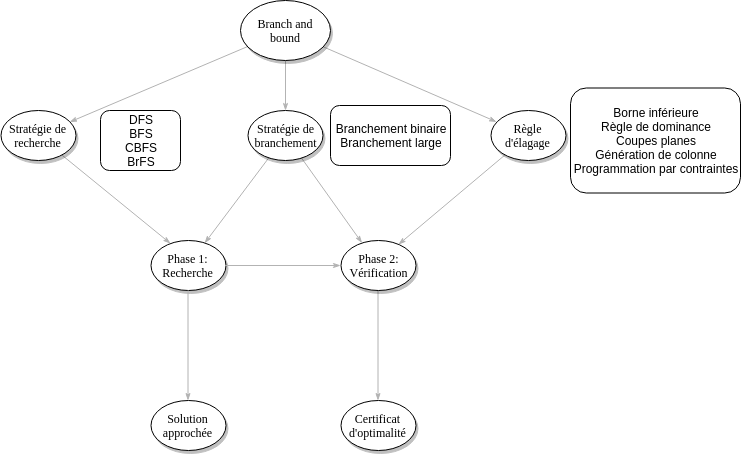
\includegraphics[width=1\linewidth]{bb_stagegies}
		\caption{Schéma résumant les trois principales composantes du Branch and bound}
		\label{fig:bbstagegies}
	\end{figure}
	\cite{MORRISON201679} divisent l'algorithme du Branch and bound en deux phases: la recherche durant laquelle on cherche une solution au problème et la vérification qui donne la preuve d'optimalité de la solution trouvée. S'il n'y a pas de preuve d'optimalité, l'algorithme fournit une solution heuristique au problème qui, dans beaucoup de cas pratiques, est suffisante. Par exemple, \cite{Morrison2014} utilisent le Branch and bound comme heuristique pour améliorer les bornes supérieures des instances. \cite{MORRISON201679} montrent sur leur schéma que la phase de recherche est beaucoup plus influencée par la stratégie adoptée pour la recherche et la politique de branchement. Alors que la phase de vérification est plus influencée par la politique de branchement et la stratégie d'élagage.
	
	\subsection{Règle d'élagage}
	L'un des aspects les plus importants de l'algorithme de branch-and-bound est la phase d'élagage. Ceci détermine les régions à éliminer de l'espace de recherche. Les règles d'élagage sont souvent spécifiques au problème traité et donc une bonne connaissance du problème est nécessaire d'autant plus que si l'on considère que la meilleure valeur pour l'élagage est la meilleure solution faisable pour le noeud et que le fait de trouver cette valeur est en sois un problème \textit{$\mathcal{NP}$-dur} \cite{Clausen99branchand} alors l'exploitation des données du problème devient crucial. \cite{MORRISON201679} classe les règles d'élagages en deux classes, celles basées sur le calcul de bornes inférieures et celle basées sur les relations de dominances.
	
	\paragraph{Le calcule des bornes}
	Il se fait en relaxant certaines contraintes du problème, la valeur générée est comparée à la meilleure solution trouvée, si elle n'est pas meilleure alors le noeud est élagué. Dans le cas des PLNE, une borne est donnée par la résolution, via la méthode du simplex par exemple, du problème sans les contraintes d'intégrité (variables continues). Ceci s'applique même pour les problèmes qui peuvent avoir une formulation en programme linéaire tel que le problème du voyageur du commerce. Mais certains problèmes tel que le problème de tournées de véhicule possède plusieurs formulations \cite{desrochers1992new} et ceci peut influer sur la qualité des bornes générées. Une autre méthode de calcul des bornes est par relaxation lagrangienne. Si on considère un problème \{$ \min f(x) \hspace{5pt} | \hspace{5pt} Ax \leq b  \hspace{5pt}, x \in \Z$ \} alors sa relaxation lagrangienne est définie par  \{$ \min f(x)- \lambda(b-Ax) \hspace{5pt} | \hspace{5pt} x \in \Z$ \}. $\lambda$ est dit multiplicateur lagrangien et c'est un vecteur de valeur négatives. La relaxation lagrangienne donne une borne inférieure du problème initial. Le problème peut être résolu avec l'algorithme du sous-gradient (\textit{Subgradient} algorithm) \cite{fisher1981lagrangian}. 
	
	\paragraph{La relation de dominance}
	Cette relation à été introduite pour la première fois par \cite{Kohler1974}. Un noeud $P_1$ est dit dominé par un noeud $P_2$ si quelque soit la solution dérivant de $P_1$, il existe au moins un solution dérivant de $P_2$ qui est au moins aussi bonne. Il suffit dans ce cas  de n'explorer que $P_2$. Il existe deux types de dominances, celle avec mémoire et celles sans-mémoire. Les dominances avec mémoire requiert de sauvegarder tous les noeuds du l'arbre branch-and-bound pour une éventuelle comparaison alors que celles sans mémoire suppose l'existance d'un problème dominant et ne requiert donc pas la sauvegarde de tous les noeuds de l'arbre. Cette méthode a été utilisée par exemple dans \cite{fischetti2010pruning} pour le cas des programmes linéaires.
	
	\subsection{Sélection du prochain sous-problème}
	La sélection du prochain sous-problème consiste à choisir le prochain noeud à explorer dans l'arbre Branch-and-bound. Il s'agit, en fait, d'une stratégie de parcours de l'arbre qui donnera l'ordre dans lequel les noeuds seront explorés. \cite{MORRISON201679} affirme que le choix de la stratégie de recherche a des conséquences significatives sur le temps de calcul nécessaire pour trouver une solution ainsi que sur la mémoire utilisée. Le choix peut aussi dépendre du problème à traiter, si un problème est difficile et consomme beaucoup de mémoire, on peut opter pour une stratégie de recherche minimisant la consommation. Par contre, si l'espace mémoire n'est pas un problème, on peut opter pour des stratégies favorisant le temps d'exécution. \cite{Ibaraki1976} donne une étude et comparaison théorique entre les stratégies de parcours et leur performances. Il regroupe toutes les stratégies sous la \textit{"Recherche Heuristique"} et donne des définitions formelles de toutes les méthodes. Ibaraki donne aussi les raisons qui font que Depth-first search (recherche en profondeur d'abord) et Best-first search ( meilleure d'abord) sont le plus souvent choisis dans la pratique. Depth-first search consomme un espace mémoire qui est fonction linéaire de la taille du problème en plus d'être facile à implémenter. Best-first search minimise le nombre de sous-problèmes à générer mais est fonction exponentielle de la taille du problème. Dans ce qui suit, on va décrire les principales stratégies de recherches utilisées dans l'algorithme Branch-and-bound.
	
	\paragraph{Depth-first search (DFS)}
	Aussi connue sous le nom de recherche en profondeur d'abord, cette stratégie explore les noeuds nouvellement générés (i.e. les noeuds fils d'un noeud en cours de branchement). Son implémention naïve se fait avec un pile contenant les sous-problèmes non encore explorés. L'algorithme choisi le noeud en haut de la pile comme prochain sous-problème à traiter et empile les noeuds fils générés dans la phase de branchement en haut de la pile. \cite{MORRISON201679} mentionne une modification qui peut être apportée à la liste des noeuds (qui peut être très grande au fil de l'avancement de l'algorithme) et réduire l'espace mémoire utilisé et ceci en introduisant une relation d'ordre entre les noeuds fils. L'algorithme DFS n'aura plus besoin de sauvegarder toute la liste des noeuds fils. On sauvegarde ainsi le chemin menant de la racine $R$ au noeud fils courant $N$. A chaque noeud fils le croisé tout au long, on sauvegarde l'index du dernier fils exploré. Le prochain sous-problème à sélectionner est donc le prochain fils non exploré. S'il n'y a plus de fils à explorer, l'algorithme remonte au noeud ancètre le plus proche possèdant des fils non encore explorés.
	
	Dans le cas des PLNE, DFS est une stratégie très employée car en plus du gain en mémoire offert par l'algorithme, on constate que les règles de branchements ne changent pas significativement la structure de la relaxation du problème entre le noeud parent et le fils, de ce fait, il est courant que dans les solveurs réutilise les informations du noeud parent comme une solution préliminaire dans les noeuds fils. Ceci étant décrit comme un \textit{démarrage à chaud} par \cite{Chinneck2004}.
	
	Néanmoins, DFS possède quelques désavantages, notamment du fait qu'il n'utilise aucune information sur la structure de problème ce qui peut  le conduire à passer beaucoup de temps à explorer une région sans succès \cite{Clausen99branchand}. Ceci peut même conduire à retarder la preuve l'infaisabilité du problème en explorant toujours plus en profondeur. Un autre désavantage surgit dans le cas d'un arbre non balancé. Si la solution optimale se trouve proche de la racine et que DFS va plus en profondeur dans l'arbre, il mettra beaucoup plus de temps à l'atteindre.
	
	DFS possède des variantes qui tentent de pallier à certains de ses désavantages, on peut citer \textit{iterative-deeping} DFS \cite{korf1985depth} qui limite la profondeur de l'arbre Branch-and-bound à explorer. Dans le cas où aucun solution optimale n'est pas trouvée, la profondeur est augmentée et la recherche recommence depuis la récine. Une autre variante est le \textit{DFS with complete branching} qui exploite les informations sur la structure du problème pour calculer les bornes inférieures des noeuds fils et sélectionne celui qui a la meilleure \cite{scholl1999balancing}.
	
	
	\paragraph{Breadth-first search (BrFS)}
	BrFS est l'opposé de DFS au lieu d'aller plus en profondeur, BrFS va en largeur et explore tous les noeuds qui sont à une même distance de la racine. Pour cela, l'implémentation se fait à l'aide d'une file d'attente. BrFS pallie au désavantage de DFS dans le cas d'arbres non balancés. La solution, si elle est proche de la racine est vite trouvée. Néanmoins, à une distance non loin de la racine, BrFS ne génère pas de bonnes bornes puisque la structure du sous-problème ne change pas beaucoup par rapport au problème initial et donc l'élagage devient tout de suite plus contraignant et l'espace mémoire pour stocker l'arbre est alors énorme. Pour pallier à cela, il faut pouvoir générer les bornes avec une heuristique. Pour ces raisons, DFS est préféré à BrFS dans la majorité des cas d'algorithmes branch and bound \cite{MORRISON201679}. 
	
	
	\paragraph{Best-first search (BFS)}
	Aussi connu sous le nom de l'algorithme $A^*$, BFS utilise une mesure $\zeta$ qui est une heuristique calculant la meilleure mesure possible pour un noeud. Cette mesure ne peut en aucun cas dépasser la fonction objectif (i.e. on ne surestime jamais la fonction objectif). Le prochain noeud à explorer est le noeud minimisant $\zeta$. Cet algorithme peut être implémenté en utilisant un tas comme structure de données. La clé d'accès au prochain noeud est $\zeta$. Le facteur le plus important est donc le choix de l'heuristique $\zeta$. Dans la programmation linéaire, c'est la relaxation du problème qui donne une borne qui peut être valeur de la fonction $\zeta$. Dans les problèmes d'optimisation, on peut introduire des fonctions qui estiment la qualité d'un noeud en se basant sur ce qui est connu du problème. L'un des avantages par rapport aux autres stratégies de recherche est que l'algorithme ne reste pas sur une branche spécifique dans l'arbre, mais explore un peu partout en se basant sur la fonction $\zeta$. L'algorithme a cependant besoin d'un espace mémoire suffisamment grand pour stocker les noeuds des sous-problème dans le tas et peu s'avérer inefficace si $k$ noeuds possèdent la même valeur $\zeta^* = \zeta(S_i) \hspace{5pt} \forall i \in 1..k$ avec $S_i$ désignant le sous-problème $i$. Ceci peut entraîner l'algorithme à intensifier l'exploration dans les régions données par $\zeta^*$ même si la solution optimale en est loin.  

     Les trois stratégies de branchement sont illustées dans les schémas suivants tiré de \cite{Clausen99branchand}. Chacun donne l'ordre d'exploration des noeuds pour chaque stratégie. Le premier est BFS, le deuxième est BrFS et le dernier est DFS. 
    %schémas expliquants l'ordre de parcours dans les 3 stratégies
    \begin{figure}[H]
		\centering
		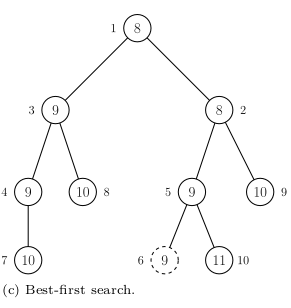
\includegraphics[width=0.5\linewidth]{BFS.png}
		\caption{Illustration du parcours BFS}
		%\label{fig:primalintegral}
	\end{figure}
	\begin{figure}[H]
		\centering
		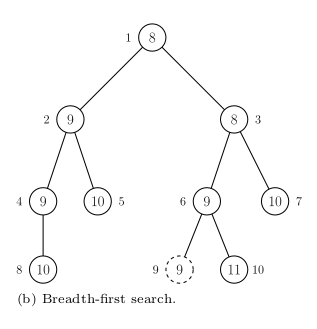
\includegraphics[width=0.5\linewidth]{BrFS.png}
		\caption{Illustration du parcours BrFS}
		%\label{fig:primalintegral}
	\end{figure}
	\begin{figure}[H]
		\centering
		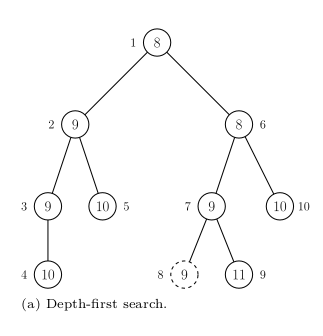
\includegraphics[width=0.5\linewidth]{DFS.png}
		\caption{Illustration du parcours DFS}
		%\label{fig:primalintegral}
	\end{figure}
	\subsection{Règles de branchement}
	La règle de branchement est la politique par laquelle l'espace des solutions est subdivisé en sous-espaces disjoints représentés chacun par un sous-problème. Ceci se fait souvent en ajoutant des contraintes additionnelles ou bien en fixant la valeur de certaines variables. La nature convergeante de l'algorithme branch-and-bound \cite{boyd2003notes} garantit que l'espace de recherche de chaque sous-problème est plus petit que celui du problème initial. \cite{MORRISON201679} classe les branchements types: les branchement binaires et les branchements larges à plusieurs noeuds.
	
	\paragraph{Les branchements binaires}
	Ce type de branchement ne génère que deux noeuds fils à chaque branchement. C'est la stratégie la plus employée dans les problèmes à variables binaires (variables ne prenant que deux valeurs: 0 ou 1). On génère un premier noeud dans lequel une première variable binaire est fixée à 0 et on génère le second noeud fils avec la même variable à 1. On peut retrouver ce cas avec le problème du sac à dos bianire (0/1 Knapsack problem) où un élément est soit ajouté dans le sac, soit complètement abandonné. D'autres problèmes tels que le problème de tournée de véhicule ou le bin packing exploitent la même idée d'inclusion et d'exclusion.
	
	\paragraph{Les branchements larges}
	Le terme branchement large (\textit{wide branching}) fut introduit pour la première fois par \cite{morrison2014wide}. Contraiement au cas binaire, la variable de branchement peut prendre plusieurs valeurs. On peut citer le cas du problème du sac à dos borné ou non borné où on doit énumérer le nombre de fois qu'on peut ajouter une variable. Chaque valeur fixée à la variable donne lieu à un sous-problème. 
	
	La phase de branchement est d'autant plus importante et très étudiée dans le cas des programmes linéaires. Les heuristiques de branchement seront, pour ce cas, abordés plus en détail dans le chapitre 2 sur les heuristiques primitives. Néanmoins, on peut citer \cite{khalil2016learning} qui utilise un modèle d'apprentissage machine à la volée (qui apprend au fur et à mesure de l'avancement dans l'arbre branch-and-bound) pour la phase de branchement. Les résultats prometteurs ainsi que la taille réduite de l'arbre généré tendent à montrer que cela peu être une piste intéressante pour de futures recherches.
	Le schéma suivant montre les deux types de branchement et les arbres qu'ils induisent.
	%dessin montant un arbre binaire et un arbre m aire pour le branchement.
	\begin{figure}[H]
		\centering
		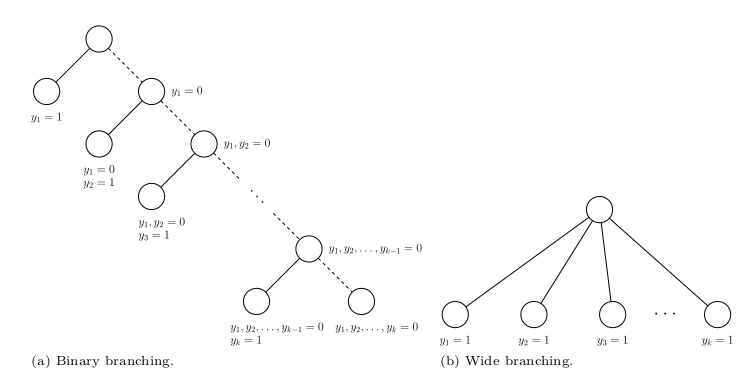
\includegraphics[width=0.9\linewidth]{binary_vs_wide.png}
		\caption{Parcours en arbre binaire vs parcours en arbre m-aire}
		%\label{fig:primalintegral}
	\end{figure}
	
	%\subsection{Le cas parallèle} 
	
	%\subsection{Exemple}
	
	
	\subsection{Application aux problèmes d'optimisation}
	Divers problème d'optimisation opte pour le branch-and-bound dans le cas d'une résolution exacte. 
	
	\paragraph{Le  problème du sac à dos non borné}
	Le problème du sac à dos est un problème de maximisation où on a $n$ objets (chaque objet $i$ est caractérisé par un gain $c_i$ et un poids $w_i$) et un sac caractérisé par un poids maximal $W$. Le but du problème est de sélectionner le nombre d'exemplaire de chaque objet $x_i$ à mettre dans le sac tout en maximisant le gain que rapporte l'objet et en ne dépassant pas le poids maximal qu'il peut porter. Le problème se formulant ainsi:
	\begin{gather}
	    \max \hspace{7pt} \sum_{i=0}^{n} c_i x_i \\
	    \text{tel que:} \hspace{15pt}
	    \sum_{i=0}^{n} w_i x_i \leq W \\
	    x_i \in \N
	\end{gather}
	Divers algorithmes et variantes du branch-and-bound on été proposées pour le résoudre. L'un des plus efficaces est celui de \cite{horowitz1974computing}. Leur algorithme commence par ordonner les objets par ordre décroissant de leur utilité (gain rapporté par unité de poids) ensuite on insère l'objet ayant la plus grande utilité dans le sac. La borne supérieure du nombre d'exemplaire de l'objet $i$ à insérer est calculée comme suit: 
	\begin{gather}
	    \floor{\frac{W-\sum_{k=0}^{i-1}w_k x_k}{w_i}}    
	\end{gather}
	Ce nombre est ensuite réduit de une unité à chaque phase de \textit{"backtracking"} pour permettre d'insérer plus d'objets d'un autre type. \cite{martello1987algorithms} changent le calcul des bornes dans l'algorithme de Horowitz et Sahni et créent un autre algorithme MT1. Ensuite ils proposent une amélioration de ce dernier avec MT2.
	
	\paragraph{Le problème du voyageur du commerce}
	 Le problème consiste à trouver le plus petit circuit de sorte que la distance parcourue soit minimale. \cite{Lawler1966BranchandBoundMA} proposent quelques applications du branch-and bound à des problème d'optimisation parmis eux le problème du voyageur du commerce. Il cite deux versions: l'algorithme de branch and bound de \cite{eastman1958linear} et celui de \cite{little1963algorithm} qui diffèrent dans les règles d'élagage. \cite{balas1983branch} proposent aussi deux version du branch-and-bound appliqué au problème du voyageur du commerce et des alternatives au calcul de bornes et pour le branchement.
	
	 \paragraph{Le problème de tournées de véhicule}
	 Ce problème peut être vu comme une généralisation du problème du voyageur du commerce où on a $m$ voyageurs au lieu de un seul. Chaque voyageur transporte avec lui une quantité $Q$ d'une marchandise et commence sa route d'un dépôt central. A chaque ville $i$, il doit livrer une quantité $q_i$ de cette marchandise. A chaque ville est associé une fenêtre de temps $[e_i,l_i]$ dans laquelle le voyageur peut arriver. Il ne peut venir ni avant $e_i$  ni après $l_i$. A chaque trajet est associé un coût. Le but étant soit de minimiser le nombre de voyageur nécessaires pour satisfaire toutes les villes soit minimiser le coût de toutes les tournée. Aucune tournée ne peut dépasser une quantité maximum $Q$ de marchandises livrées. \cite{kolen1987vehicle} proposent un algorithme de branch-and-bound pour résoudre le problème de tournées de véhicules avec fenêtre de temps. Chaque noeud correspond à un ensemble de tournées commençant et finissant au dépôt. Ils créent ensuite un ensemble de routes partielles initialisées au dépôt et leur associent une liste de villes interdites à visiter. La phase de branchement consiste à sélectionner une ville $j$ qui n'apparaît dans aucune route, ni dans la liste des routes interdites selon un heuristique donnée par \cite{kolen1987vehicle}. Deux noeuds sont alors crées: un noeud avec la route partielle contenant la ville $j$ et une autre ne où $j$ apparaît dans la liste des villes interdites à visiter. Kolen et al. donnent ensuite les inégalités nécessaires pour générer les bornes inférieures et supérieures. Une revue des algorithmes branch-and-bound appliqués au problème de tournées de véhicule peut être retrouvé dans \cite{toth2002branch}.     
	
	%\subsection{Avantages et inconvénients}
	
	
	\section{Branch and cut}
	\subsection{Méthode des plans sécants} \label{plansec}
		\subsubsection{Description de la méthode}
		La méthode des plans sécants est un méthode qui vient de la programmation en nombre entier. Ils furent introduit pour la première fois par 
		\cite{gomory1958outline}. Leur inconvénient était la convergence lente de ces algorithmes ce qui fait qu'ils ont été délaissés pendant un bon moment avant d'être repris dans les années 1980. Avant de décrire l'algorithme, quelques définitions tirées de \cite{fukuda2000} sont nécessaires pour comprendre la suite.
		
		\begin{definition}\
            Soient $a,x \in \R^n$ , $b \in \R $, $A \in \R^{m \times n}$ une matrice $m \times n$ et $c \in \R^{m \times 1}$ un vecteur. On défini alors:
            \begin{itemize}
                \item Un demi-espace est l'ensemble des points $x$ telle que $a \cdot x \leq b $.
                \item Un polyhèdre est l'intersection d'un ensemble fini de demi-espaces. (i.e. c'est l'ensemble $\{x \hspace{5pt} | \hspace{5pt} Ax \leq c \}$
                \item Un polytope est un polyhèdre borné.
                \item L'enveloppe convexe d'un ensemple $S \in \R^n$ est l'intersection de toutes les parties convexes de $\R^n$ contenant $S$.
                \item Une facette d'un polytope de dimention $n$ est une face de dimention $(n-1)$
            \end{itemize}
        \end{definition} 
        
        \begin{definition} \
            Une coupe sécant est une contrainte qui peut être ajoutée à un programme en nombre entier pour restreindre la région des solutions faisables sans éliminer aucune solution entière. \cite{MORRISON201679}
        \end{definition}
		     L'algorithme vise donc résoudre la relaxation d'un programme linéaire qui, dans le cas général, ne donne pas la solution entière. Dans le cas où la relaxation est infaisable le programme en nombre entier l'est aussi. Dans les autres cas, l'algorithme cherche des coupes au moyens de procédures générales ou tenant compte de la structure du problème et les ajoute pour restreindre la région des solutions entières et éliminer celles qui ne le sont pas.
		\subsubsection{Pseudocode}
		%donner des explications sur l'algo 
	    \begin{algorithm}[H]
		    \caption{Algorithme des plans sécants}
    		\SetAlgoLined
    		\DontPrintSemicolon
    		\textbf{Entrée:} $P$ le problème initial \;
    		\textbf{Sortie:} Solution, ValeurOptimale \;
    		
    		résoudre la relaxation $\bar{P}$ de $P$ \;
    		\If{$\bar{P}$ est infaisable}
    		{
    		    retourner "Infaisable" \;
    		}
    		\If{ $\bar{P}$ donne une solution entière $S^* = f(x^*)$}
    		{
    		    Solution $\gets$ $S^*$ \;
    		    ValeurOptimale $\gets$ $x^*$ \;
    		    retrouner (Solution, ValeurOptimale) \;
    		}
    		\If{au moins une des variables de $x^*$ est fractionnelle}
    		{
    		    Chercher et ajouter une ou plusieurs plans sécants qui séparent $x^*$ de l'enveloppe convexe des solutions entières faisables \;
    		    Aller à 3 \;
    		}
	    \end{algorithm}
		%\subsubsection{Exemples}
		\subsubsection{Type de coupes existants}
		\paragraph{Coupes de Chvatal et Gomory:}
		Ces coupes ont été décrites dans \cite{gomory1958} et \cite{CHVATAL1973305}. Elles combinent des inégalités issues de la relaxation du programme linéaire. Gomory extrait les contraintes en utilisant le tableau optimal de la méthode du simplex à partir d'une de ses lignes. La convergence de cet algorithme est lente. Il existe des techniques pour accélérer la convergence, par exemple, en rajoutant plusieurs coupes à la fois. \cite{mitchell2009integer} affirme que la convergence de l'algorithme des coupes sécants implique que chaque inégalité valide pour l'enveloppe convexe est soit générée en arrondissant les variables ou bien par domination par une inégalité. Il définit ensuite \textit{le rang de Chvatal} d'une inégalité comme étant le nombre minimal d'application successives d'arrondissements nécessaires pour la générer. Les inégalités de rang 2 peuvent être générées en appliquant une méthode d'arrondissement à un large nombre d'inégalités de rang 0 et 1. Le rang donne une mesure de la complexité de l'enveloppe du polytope. 
		%todo: rajouter un exemple.
		
		\paragraph{Les coupes de cliques}
		Une clique est un ensemble de variables incompatibles. En terme ensembliste, cela donne:
		$C=\{x \in B \hspace{5pt}| \hspace{5pt} x_i  \hspace{5pt} \text{et}  \hspace{5pt} x_j  \hspace{5pt} \text{sont incompatibles}\}$
		Un groupe de variables sont dites incompatibles si au maximum, seule l'une d'elle peut être positive. Par exemple: $x+y \leq 1$ implique que soit $x=1$ et $y=0$ ou bien l'inverse. 
		Une coupe de cliques est une inégalité se basant sur les l'incompatibilité des variables. Elle prend la forme générale de $\sum_{j \in C} x_j \leq 1 $. Cette inégalité est principalement utile pour les problèmes qui font apparaître des clique non désirées dans les solution. Par exemple, on peut les envisager pour l'élimination des sous-tours comme dans le cas du problème du voyageur du commerce \cite{HERNANDEZPEREZ2004126}.
		Les solveurs tels que CPLEX incluent aussi ce type de coupes. Par exemple, CPLEX s'en sert avant le début de l'optimisation et génère à partir de toutes les coupes de ce type un graphe et ensuite essayer de trouver les cliques maximales dans le graphe.
		
		\paragraph{Lift-and-project}
	    Soit un problème binaire $S := \{ x: Ax \leq b, x_i = 0, 1, \forall i \}$.
		Chaque variable peut être utilisée pour générer un ensemble disjoint. Soit
        \begin{gather}
            S_j^0 := \{ x: Ax \leq b, 0 \leq x_i \leq 1, \forall i, x_j = 0 \}
        \end{gather}
         et
         \begin{gather}
             S_j^1 := \{ x: Ax \leq b, 0 \leq x_i \leq 1, \forall i, x_j = 1 \}
         \end{gather}
         Alors $S \subseteq S_j^0 \cup S_j^1$, d'où le fait que des inégalités valides pour $S$ peuvent être générées en trouvant des inégalités pour l'enveloppe convexe de $S_j^0 \cup S_j^1$ \cite{mitchellbranch}. Ces inégalités sont générées à résolvant des programmes linéaires associés décrits dans \cite{bonami2012optimizing}. Cette disjonction n'est valable que pour le cas de variables entières ce qui permet d'éliminer les variables fractionnelles générées lors des relaxations.
		
	    Un autre exemple de ce type de disjonction qu'on peut retrouver dans le solveur CPLEX \cite{manual1987ibm}:$dx \leq d_0$ ou $dx \textgreater \d_0 +1$
	    
		Cette inégalité crée les deux sous problèmes:
		\begin{gather}
		    P_1 = \{ x \in P \hspace{5pt} | \hspace{5pt} dx \leq d_0 \}
		\end{gather}
		et
		\begin{gather}
		    P_2 = \{ x \in P \hspace{5pt} | \hspace{5pt} dx \textgreater d_0 +1  \}    
		\end{gather}
		
		\subsubsection{Application aux problèmes d'optimisation}
		
		La méthode des plan sécants a été appliqué à bon nombre de problèmes d'optimisation. Par exemple, dans le cas du problème du voyageur du commerce, on peut citer \cite{grotschel1991solution} qui donne une procédure de plan sécants capables de résoudre à l'optimalité le problème pour 1000 villes. \cite{miliotis1978using} développe aussi deux algorithmes de plan sécants qui commencent par un sous-ensemble des contraintes du problème originel. Les deux diffèrent dans l'ordre dans lequel les contraintes omises et les plan sécants sont générées.
		\cite{cook1999parallel} proposent une adaptation parallèle des plan sécants inspirée de l'algorithme de Karger pour le problème de tournées de véhicules avec fenêtre de temps suivi d'une méthode branch-and-bound.
		
		
		%\subsubsection{Avantages et inconvénients}
		
	\subsection{Le branch and cut}
	
		\subsubsection{Description de la méthode}
		
		Le branch-and-cut est une méthode exacte de résolution de problèmes pour les programmes en nombres entiers. C'est une combinaison de la méthode des plan sécants et du branch-and-bound. Le principe est de résoudre une séquence de relaxation de programmes linéaires et se servir des plans sécants pour améliorer la relaxation pour restreindre l'espace des solution à celui des solutions entières telle que vu dans \ref{plansec} et branch-and-bound opère avec une procédure sophistiquée de type \textit{diviser pour régner} pour décider du prochin sous-problème à traiter. Tous les concepts vus pour le branch-and-bound dans \ref{bb} sont valables pour le branch-and-cut. 
		L'algorithme peut être précéde d'une phase de pré-traitement dans laquelle le nombre de variables du problème peut être réduit et quelques contraintes éliminées. C'est le cas de l'algorithme de branch-and-cut implémenté dans le solveur CPLEX \cite{manual1987ibm}.
	
	    Le coût de l'introduction des plans sécants peut être énorme.  De ce fait, il est essentiel d'établir un stratégie pour le moment de cherche des coupes à ajouter et de ne pas le faire dans tous les noeuds de l'arbre branch-and-bound. Pour cela, on peut opter pour ajouter les coupes tous les $n$ noeuds visités ou bien à la profondeur $n$ ou une combinaisons d'autres paramètres.
		
		\subsubsection{Algorithme général}
		%donner des explications sur l'algo 
		
		\cite{mitchellbranch} donne l'algorithme général du branch-and-cut.
		
		\begin{algorithm}[H]
		    \caption{Algorithme Branch-and-cut}
    		\SetAlgoLined
    		\DontPrintSemicolon
    		\textbf{Entrée:} $P_0$ le problème initial \;
    		\textbf{Sortie:} Solution, ValeurOptimale \;
    		\textbf{Initialisation:} $L \gets \{P_0\}$, $\bar{z} \gets +\infty$, $\underline{z} \gets -\infty$ \;
    		\textbf{Terminaison:}\;
    		    \If{$L = \emptyset$}
    		    {
    		        \eIf{$\bar{z} = +\infty$}
    		        {
    		            retourner "Infaisable" \;
    		        }
    		        %else
    		        {
    		            Solution $\gets \bar{z}$ \;
    		            ValeurOptimale $\gets x^*$ avec $\bar{z} = f(x^*)$, $f$ étant la fonction objectif\;
    		        }
    		    }
    		\textbf{Sélection d'un noeud:}\;
    		    Sélectionner et supprimer un noeud $P_i \in L$ \; 
    		\textbf{Relaxation:} \;
    		    Résoudre la relaxation de $P_i$\;
    		    \eIf{la relaxation de $P_i$ est infaisable}
    		    {
    		        $\bar{z} \gets +\infty$ \;
    		        Aller à Elagage \;
    		    }
    		    %else
    		    {
    		        $\underline{z} \gets$ \begin{cases}
    		                                     $f(\underline{x})$  & \text{dans le cas où c'est une solution finie}\\
    		                                     -\infty & \text{sinon}
    		                              \end{cases} \;
    		        
    		        
    		    }
    		\textbf{Ajout de plans sécants:} \; \\
    		    \If{Condition d'ajout respectée}
    		    {
    		        Chercher des plans sécants qui sont violées par la solution $\underline{x}$ et les ajouter à la relaxation \;
    		        \If{Il y a des plans sécants}{
    		            Aller à Relaxation \;
    		        }
    		    }
    		    
    		 \textbf{Elagage:}\;
    		    \If{\underline{z} \geq \bar{z}}
    		    {
    		        Aller à Terminaison \;
    		    }
    		    \If{\underline{z} \textless \bar{z} et $\underline{x}$ est entière}
    		    {
    		        $\bar{z} \gets \underline{z}$ \;
    		        Supprimer de $L$ tous les problèmes avec $\underline{z} \geq \bar{z}$ \;
    		        Aller à Terminaison \;
    		    }
    		 \textbf{Branchement:} \;
    		 Partitionner l'espace $S\textsuperscript{i}$ des solutions associé à $P_{i}$ en $k$ espaces $\{S\textsuperscript{ij} \}_{j=1}^{j=k}$ \;
			 $ L \gets L \bigcup \{P_{ij} \}_{j=1}^{j=k}$ \;
			 $\underline{z}_{ij} \gets \underline{z}$ \hspace{10pt} $ \forall j \in \{1..k\} $ 
		\end{algorithm}
		L'algorithme est le même que celui du branch-and-bound pour le cas des PLNE excepté qu'une phase de génération de plans sécants est ajouté. Généralement cette phase dit de \textit{"cut"} génère un énorme nombre de contraintes et souvent un sous-ensemble de ces contraintes seulement est pris en considération. Les contraintes générées peuvent alors être triées selon un critère telle que le nombre de violations. Généralement, ce sont les coupes de Gomory et Chvatal qui sont le plus employées. Les coupes générées par \textit{lift-and-project} peuvent être employées elles aussi, mais comme le fait remarquer \cite{mitchellbranch} elles sont coûteuse au niveau de la racine et donc sont laissées au milieu pour les noeuds fils. Deux type de plans sécants peuvent être considérés dans l'algorithme, les plans qui sont généraux et qui peuvent s'appliquer à tous les noeuds de l'arbre et les plans locaux propres à un noeuds et qui ne sont valides que pour lui et ses descendants. Ce dernier type de noeud peut présenter des désavantages quant à la consommation mémoire que requière la sauvegarde de versions différentes du problème. Ces plans ne sont donc pas privilégiés, c'est la cas par exemple du solveur CPLEX qui s'efforce de trouver des plans sécants valables pour tous les noeuds \cite{manual1987ibm}. 
		
		%\subsubsection{Exemples}
		
		\subsubsection{Application aux problèmes d'optimisation}
		Le branch-and-cut est une des techniques qui remporte le plus de succès pour la résolution d'un large éventail de problèmes. On peut citer, par exemple, pour le problème du voyageur du commerce \cite{padberg1991branch} qui a résolu de larges instances avec optimalité en utilisant un algorithme branch-and-cut avec des coupes tirées de la théorie des polyhèdres.
		\cite{bixby1998solving} a réussi à employer la méthode pour le problème de tournées de camions pour lequel des contraintes de type sac à dos ont été employées. \cite{hoffman1993solving} résout le problème de planification de vols aériens. Les plans sécants sont générés en exploitant la structure du polytope défini par l'enveloppe convexe des points entiers. \cite{bard2002} utilise le branch-and-cut dans le cas du problème de tournées de véhicules avec fenêtre de temps avec comme objectif principal la réduction du nombre de véhicules et introduit plusieurs types d'inégalités d'inégalités à partir des travaux sur la variante sans fenêtre de temps, puis expose les inégalités avec fenêtre de temps.
		
		%\subsubsection{Avantages et inconvénients}
		\subsection{Variante}
		Si on ajoute les plans sécants au noeud racine dans un arbre branch-and-bound, la méthode est dire \textit{cut-and-branch}. Comme souligné précédemment, l'ajout de plans à la racine nécessite plus de calcul et plus de temps pour la résolution, ce qui représente un grand désavantage de la méthode. Autre désavantages, est le fait qu'elle ne donne pas de bons résultats sur des instances durs de problèmes spécifiques contrairement au branch-and-cut qui a prouvé son efficacité. Néanmoins, \cite{mitchellbranch} cite quelques avantages:
		\begin{itemize}
		    \item Tous les plans sécants générés sont valides dans tout l'arbre branch-and-bound,
		    \item Gain de temps au fait de ne pas générer d'autres plans sécants dans les autres noeuds de l'arbre,
		    \item Réduction du nombre de noeuds à sauvegarder, puisque les relaxations sont identiques à chaque noeud de l'arbre. 
		\end{itemize}
		

	\section{Branch and price}
	
	    
		\subsection{Méthode de génération de colonnes}
			
			Selon \cite{nemhauser2012column} c'est Fulkerson et al. qui ont introduit la méthode de génération de colonne bien que le terme n'apparaît pas explicitement dans leur papier \cite{fulkerson1971blocking}. 
			
			Dans la méthode de génération de colonnes, on introduit deux problèmes issus du problème initial. \cite{desrosiers2010branch}
			Le problème \textit{maître} (master problem) défini par :
			\begin{gather}\label{master_prob}
			    \min \sum_{j \in J} c_j \lambda_j \\
	        \end{gather}
			tel que: 
			\begin{gather*}
			    \sum_{j \in J} a_j \lambda_j \geq b \\
			    \lambda_j \geq 0, j \in J
			\end{gather*}
			 
			 A chaque itération, on chercher une variable hors base à faire entrer dans la base. On associe pour cela au problème maître un problème dit de \textit{pricing} défini comme suit.
			 Soit $u \geq 0$ un vecteur des variables duales, on veut trouver 
			 \begin{gather}\label{argmin_cg}
			     \textit{arg}\min \{ \bar{c}_j := c_j - u^T a_j \hspace{5pt} | \hspace{5pt} j \in J \}
			 \end{gather}
			 Si $|J|$ est grand, le calcul \ref{argmin_cg} devient impossible et on ne travaille qu'avec un sous ensemble $J' \subseteq J$ de varaibles. Le problème maître est alors désigné comme étant un problème maître restreint (RMP).  
			 Soit $A$ un ensemble contenant des colonnes $a_j$, $j \in J$. On défini alors le sous-problème
			 \begin{gather} \label{oracle}
			     \bar{c} := \min \{ c(a) - u^T a \hspace{5pt}| \hspace{5pt} a \in A \}
			 \end{gather}
			 C'est le sous-problème qui donne la solution au problème de \textit{pricing} et qu'on appel par le coût réduit. Si $\bar{c} \geq 0$ alors $\bar{\lambda}$ résout le problème maître. Dans l'autre cas ($\bar{c} \textless 0$), on ajoute au problème maître restreint la colonne donnée en sortie par \ref{argmin_cg} et minimisant \ref{oracle}
			 
			 Dans le cas des programmes linéaire, \cite{dantzig1960decomposition} introduisent leur décomposition. Le programme initial étant sous la forme:
			 
			 \begin{gather*}
			    \min c^T x \\
	        \end{gather*}
			tel que: 
			\begin{gather*}
			    Ax \geq b \\
			    Dx \geq d \\
			    x \geq 0
			\end{gather*}
			
			On considère 
			\begin{gather}\label{Xprob} 
			    X := \{ x \in \Z_+^n \hspace{5pt}|\hspace{5pt}Dx \geq d \}    
			\end{gather}
			comme état un problème "relativement facile" à résoudre et le problème
			 \begin{gather*} \label{MinProb}
			    \min c^T x \\
	        \end{gather*}
			tel que: 
			\begin{gather*}
			    Ax \geq b \\
			    x \geq 0
			\end{gather*}
			"relativement difficile" à résoudre.
			
			Suivant la formulation donnée dans \cite{desrosiers2010branch}, on fait la \textit{convexification} du problème \ref{Xprob}. Chaque $x \in X$ peut être représenté comme une combinaison convexe d'un nombre fini de points $\{x_p\}_{p \in P}$ et d'un nombre fini de raies $\{x_r\}_{r \in R}$ issues de $conv(X)$ l'enveloppe convexe de $X$.
			\begin{gather}
			    x = \sum_{p \in P} x_p \lambda_p  + \sum_{r \in R} x_r \lambda_r \\
			    \sum_{p \in P} \lambda_p \\
			    \lambda \in \mathbb{Q}^{|P|+|R|}
			\end{gather}
			
			Si on substitue dans \ref{MinProb} et qu'on change $c_j = cx_j$ et $a_j = Ax_j$ pour $j \in R \cup P $, on obtient le problème maître:
			\begin{gather} \label{master_pb}
    			\min \sum_{p \in P} c_p \lambda_p + \sum_{r \in R} c_r \lambda_r \\
    		\end{gather}
    		telle que:
    		\begin{gather*}
    		    \sum_{p \in P} a_p \lambda_p + \sum_{r \in R} a_r \lambda_r \leq b \\
    		    \sum_{p \in P} \lambda_p =1 \\
    		    \lambda \geq 0 \\
    		    x = \sum_{p \in P} x_p \lambda_p + \sum_{r \in R} x_r \lambda_r \\
    		    x \in \Z_+^n
    		\end{gather*}
    		
			La cardinalité de $P \cup R$ étant grande le problème maître est résolu \ref{master_pb} par la méthode de génération de colonne. Le problème de pricing associé au maître est
			\begin{gather}
			    \min \{ cx - \pi Ax - \pi_0 | x \in X \}
			\end{gather}
			avec $\pi$ étant les variables duales et $\pi_0$ la contrainte de convexité.
			
			%\subsubsection{Description de la méthode}
			%\subsubsection{Algorithme général}
			%donner des explications sur l'algo 
			
			%\subsubsection{Exemples}
			
			%\subsubsection{Application aux problèmes d'optimisation}
			
			%\subsubsection{Avantages et inconvénients}
			
		\subsection{Le branch and price}
		
			\subsubsection{Description de la méthode}
			Branch-and-price peut être vu comme l'algorithme dual du Branch-and-cut. Si dans le branch-and-cut on s'interesse à générer des contraintes (et donc des lignes) pour le problème, dans branch-and-price, on s'interesse aux variables (et donc les colonnes)
			Le principe du branch-and-price est de ne pas utiliser des colonnes (variables) dans la relaxation du problème. Deux éléments justifient cette approche: le fait qu'il y a beaucoup de variables dans la formulation du problème et une observation sur le fait que la plupart des variables dans la solution optimale sont mises à 0. Deux sous-problèmes sont générés, le \textit{pricing problem} qui essai d'identifier les colonnes à ajouter. Si des colonnes sont trouvées le programme linéaire est réoptimisé, sinon on passe à la phase de branchement. A chaque noeud du branch-and-price, l'algorithme fait appel à la méthode de génération de colonne. 
			
			Bien que l'idée du branch-and-price peut paraître simple si on se dit qu'on ne fait qu'un hybridation d'une méthode de génération de colonnes dans un branch-and-bound, néanmoins, \cite{savelsbergh2001branch} souligne la non-trivialité de la chose et ceci pour les prinicpales raisons suivantes:
			\begin{itemize}
			    \item Les règles de branchement connues pour les programmes linéaires peuvent ne pas être effective car fixer des variables peut détruire la structure du problème de \textit{pricing}
			    \item La méthode de génération de colonne converge lentement vers la solution optimale et peut donc devenir un goulot d'étranglement pour tout l'algorithme
			\end{itemize}
			
			
			
			\subsubsection{Algorithme général}
			%donner des explications sur l'algo 
			
			
		\begin{algorithm}[H]
		    \caption{Algorithme Branch-and-price}
    		\SetAlgoLined
    		\DontPrintSemicolon
    		\textbf{Entrée:} $P_0$ le problème initial \;
    		\textbf{Sortie:} Solution, ValeurOptimale \;
    		
    		Formuler le problème maître de $P_o$ tel que dans \ref{master_prob}  \;
    		Extraire le problème maître restreint (RMP)\;
    		Résoudre le problème de \textit{pricing} \;
    		\eIf{le coût réduit ( défini dans\ref{oracle}) < 0}
    		{
    		    Ajouter la colonne trouvée au RMP \;
    		    Aller à 4 \;
    		}
    		{
    		    \eIf{solution entière trouvée}
    		    {
    		        retourner Solution, ValeurOptimale;
    		    }
    		    {
    		        Appel à la procédure de branchement \;
    		        Aller à 4
    		    }
    		}
    		
    	\end{algorithm}
			
		La procédure de branchement est la plus délicate dans l'algorithme car elle peut interférer avec la structure du problème de pricing initial c'est pour cela que la plupart des algorithmes branch-and-price utilisent des branchement alternatifs. Beaucoup existent dans la littérature tels que dans la coloration de graphe \cite{Mehrotra1996} et le problème d'affectation généralisé \cite{Savelsbergh1997}. Le banchement est traité plus en détail dans \cite{vanderbeck2011branching}
		%\subsubsection{Exemples}
		
		
		\subsubsection{Application aux problèmes d'optimisation}
		L'algrithme de branch-and-price ainsi que la génération de colonne est utilisée pour résoudre des problèmes ayants une formulation en problème de partitionnement \cite{archetti2014survey}. C'est le cas par exemples des problèmes de tournées de véhicules tels que \cite{dell2006branch}, \cite{feillet2010tutorial}, \cite{danna2005branch}, \cite{christiansen2007branch} et \cite{salani2011branch}
		Le problème de coloration de graphes \cite{hoshino2011branch}, \cite{Mehrotra1996}, \cite{archetti2014branch}.
		%\subsubsection{Avantages et inconvénients}
			
		%\subsection{Cas particuliers}
		
			%branch and cut and price
			 
			
			%branch and price and cut
	
	
	
	\section{Conclusion}
    
    Nous avons vu dans ce chapitre les méthodes de résolution exactes et plus précisément les méthodes arborescentes. Le branch-and-bound qui constitue la méthode pilier des autres méthodes. Nous avons vu que c'était plus un \textit{framework} qu'il offrait tant il y a des déscisions, des heuristiques et des méthodes applicables à toutes les étapes importantes. Que ce soit pour l'initialisation, le branchment, le calcul des bornes, la stratégie d'élagage ou le choix du prochain sous-problème, faire varier un seul de ses paramètres permet d'inflencer le cours de l'exécution de l'algorithme. Les application de celui-ci sont légion, que ce soit pour les programmes linéaires ou bien pour des problèmes d'optimisation plus spécifiques tel que le problème du voyageur du commerce, la coloration de graphe ou d'autres, le branch-and-bound a prouvé être l'une des meilleures méthodes exacte pour la résolution. Une amélioration du branch-and-bound est le branch-and-price qui exploite la méthode des plans sécants introduits par Gomory et Chvatal et qui permet de restreindre l'espace des solution et de l'affiner pour se rapprocher de la couverture convexe. Le défi dans cette méthode est de trouver les contraintes à rajouter dans le programme linéaire pour de sorte à ce qu'elles soient valables dans tous les noeuds de l'arbre. La méthode à été appliquée à presque tous les problèmes d'optimisation pourvu qu'une formulation en programme linéaire est disponible. Enfin, la dernière méthode arborescente présentée est celle du branch-and-price. On a vu qu'elle est plus délicate que les autres méthodes du fait qu'il faut développer des méthodes de branchement spécifiques qui font attention à ne pas altérer la structure du problème de \textit{pricing}. Ses utilisations sont concentrées principalement sur les problèmes qui peuvent se formuler en problème de partitionnement notamment les problèmes de tournées pour laquelle elle consistitue l'une des méthdoes les plus performantes de la littérature.
    
    Le branch-and-bound et ses variantes peuvent encore être améliorés sur toutes les phases. Nous pourrons voir ceci dans le chapitre 2 sur les heuristiques primitives qui donnent des politiques de branchement et de sélection du prochain sous-problème plus élaborées et généralisées au programmes linéaires.   


	\chapter{Les heuristiques primitives}
	
	\section{Introduction}
	Le programmation mathématique est une branche des techniques d’optimisation d’une grande utilité pour la résolution exacte d’un problème de maximisation ou de minimisation.  Beaucoup de problèmes d’optimisation peuvent se formuler en un programme mathématique tels que les problème de transport, de réseaux de télécommunication, ordonnancement, etc.\cite{Gamrath2015}. Il est donc intéressant de pouvoir exploiter cette structure pour la résolution du problème, d’où un intérêt pour trouver des algorithmes de résolution des programmes mathématiques. Toutefois, en raison du nombre important de variables, le temps d’exécution peut vite exploser et passer de quelques secondes à des heures voir des années. En particulier, on parle plus de programmation linéaire avec toutes ses variantes : en nombres entiers, en nombre mixtes (variables entières et réelles), en nombres binaires (variables prenants seulement 0 ou 1 comme valeurs). Le cas non-linéaire est discuté dans \cite{berthold2014heuristic}.
	
	\paragraph{}
	Les heuristiques primitives sont un aspect important de la programmation linéaire. Ces heuristiques permettent de générer des solutions faisables de bonnes qualité en des temps d’exécution relativement courts ou d’améliorer une solution trouvée pour la rapprocher de l’optimalité. Ces heuristiques sont propres au domaine de la programmation mathématique et nécessite donc de trouver une formulation en programme linéaire du problème qu’on souhaite minimiser (ou maximiser) pour pouvoir les appliquer. 
	
	\paragraph{}
	Beaucoup de solveurs commerciaux et open-source tels que SCIP ou IBM CPLEX proposent des implémentations des heuristiques primitives et font appel à elles au cours de la résolution des programmes linéaires. Dans \cite{Berthold2018}, Berthold donne les résultats de tests sur des benchmarks de la littérature dans lesquels il montre l’impacte des heuristiques  primitives sur l’accélération de la résolution des programmes linéaires. 
	
	\paragraph{}
	Dans ce qui suit, on va d’abord faire un rappel sur quelques notions de la programmation linéaire. Notamment la définition d’un programme linéaires, les types de programmes linéaires et la définition d'une solution dite \textit{"faisable"}. Puis, on va aborder les heuristiques primitives en se basant principalement sur les travaux de Achterberg et Berthhold \cite{berthold2006}. On suivra la même classification qui y est proposée. Enfin, on présentera quelques résultats de tests sur l'efficacité de ces heuristiques.
	
	\section{Rappels sur les programmes linéaires}
	\paragraph{}
	\textit{Dans ce qui suit, nous allons donner les définitions les plus importantes qui reviennent tout au long de l’étude des heuristiques primitives. Ces définitions peuvent être retrouvées notamment dans \cite{berthold2006} et \cite{Hendel2011}. %Pour les notions de générations de colonnes et de branch-and-bound et ses variantes, il faut se référer au chapitre [chapNum]. 
	}
	
	\begin{definition} \label{def:defmip} \ 
		Soit $m,n \in \N, A \in \R^{m \times n}, b \in \R^m, c \in \R^n, l,u \in \R^n et I \subset N := \{1,...,n\} $
		On appelle:\\
		
		\[
		\begin{aligned}
		\text{min} \hspace{10pt}  c^T x \\
		\text{telle que:} \hspace{10pt} Ax \leq b \\ 
		l \leq x \leq u \\
		x_j \in \mathbb{Z} \hspace{10pt} \forall j \in I \\
		x_j \in \R \hspace{10pt} \forall j \notin I 
		\end{aligned}
		\]
		
		
		un programme linéaire en nombre mixte (MIP).
	\end{definition}
	
	\begin{itemize}
		\item[$\circ$] $c^T x$ est appelée fonction objectif. Dans notre cas, on considère un problème de minimisation.
		\item[$\circ$] $A x \leq b$ sont les contraintes linéaires 
		\item[$\circ$] $u$ et $l$ sont des contraintes de bornes.  $u$ étant la borne supérieure et $l$ la borne inférieure. Si de plus, on définit $B := \{j \in I \hspace{5pt}|\hspace{5pt} l_j = 0 \hspace{5pt} \text{et} u_j = 1 \hspace{5pt} \}$, alors les variables $x_j, j \in I$ sont des variables binaires.
		\item[$\circ$] $x \in \Z  $ est la contrainte d'intégrité du MIP
		\item[$\circ$] On peut toujours assumer que les bornes sont dans $\Z$ puisque $x \in \Z $. Si la borne supérieur $u$ est fractionnelle, on arrondira à l’entier directement inférieur $\floor{u}$ . Si par contre la borne inférieure $l$ est fractionnelle, on arrondira à l’entier directement supérieur $\ceil{l}$. 
		\item[$\circ$] $P(A,b,l,u)$ désignera l'ensemble des points $x$ solution du MIP  ~\ref{def:defmip}
	\end{itemize}

	\begin{definition} \
			Un MIP est dit:\\
			\begin{itemize}
				\item[$\circ$] Programme linéaire (LP) si $I = \emptyset$
				\item[$\circ$] Programme  en nombre entier (IP) si $ I = N $
				\item[$\circ$] Programme en nombres binaires (BP) si $ I = B = N $
				\item[$\circ$] Programme mixte en nombres binaires si $ I = B $
				
			\end{itemize}
	\end{definition}
	
	\begin{definition} \ 
		
		Soit $\hat{x} \in \R^n$. On appelle $\hat{x}$ une solution:\\
		\begin{itemize}
			\item[$\circ$] LP-faisable pour (1.1) si $A\hat{x} \leq b \hspace{5pt} \text{et} \hspace{5pt} l \leq \hat{x} \leq u$ 
			\item[$\circ$] Entière faisable pour (1.1) si $\hat{x_j} \in \N \hspace{5pt} \forall j \in I$ 
			\item[$\circ$] Faisable pour (1.1) si $\hat{x}\hspace{5pt} \text{est LP-faisable et entière faisable} $ 
			\item[$\circ$] Optimale faisable pour (1.1) si $\hat{x} \hspace{5pt} \text{est faisable et } \hspace{5pt} c^T\hat{x} \leq c^Tx \hspace{5pt}\\
			\text{pour toutes autre solution faisable x}$
		\end{itemize}
		
	\end{definition}

	\begin{definition}
		La LP-relaxation d’un programme linéaire est défini à partir du programme de la définition 1.2.1 en omettant les contraintes d’intégrité. De façon plus formelle :
		\begin{equation}
			\begin{aligned}
				\text{min} \hspace{10pt}  c^T x \\
				\text{telle que:} \hspace{10pt} Ax \leq b \\ 
				l \leq x \leq u \\
			\end{aligned} 
		\end{equation}
		Notons que cela correspond aussi à la définition de programme linéaire (LP) dans 1.2.2 puisque dans ce cas, on force $I = \emptyset$
		
	\end{definition}


	\section{Les heuristiques primitives}
	\subsection{Définition}
	Selon \cite{Lee2001}: \textit{"The term primal heuristics refers to certain LP-based procedures for constructing integral feasible solutions from points that are in some sense good, but fail to satisfy integrality. Typically, these nonintegral points are obtained as optimal solutions of LP relaxations. Primal heuristic procedures involve successive variable fixing and rounding (according to rules usually governed by problem structure) and subsequent resolves of the 			modified primal LP".}
	\paragraph{}
	Les heuristiques primitives sont donc des heuristiques appliquées aux MIPs. Elles visent à trouver des solutions de bonnes qualités sans pour autant garantir l’optimalité. Les premiers travaux sur les heuristiques pour les programmes linéaires sont dus à \cite{gomory1958}. Une heuristique appelée Pivot-and-complement à aussi été proposée par Balas et Martin pour les programmes en nombres binaires (BP) \cite{Balas1980}. Le principe du pivot est basé sur l’observation qu’une solution faisable est une solution de la relaxation du programme linéaire où les variables binaires sont hors bases (en utilisant la méthode du simplexe) et donc les variables d’écart seulement sont basiques. L’heuristique de pivot essaie donc de transformer un maximum de variables binaires en variables hors base tout en gardant le solution faisable et en altérant le moins possible la fonction objectif. Par la suite, l’heuristique a connu plusieurs améliorations et une généralisation pour les programmes linéaires en nombres mixtes. Dans la suite, nous nous intéresserons aux heuristiques primitives implémentées dans les solveurs tel que SCIP.
	
	\paragraph{}
	\cite{Hendel2011} cite certaines heuristiques triviales. Celles-ci sont des heuristiques directes qui n'ont pas besoin de beaucoup de calculs et appliquent une logique plutôt simple. Hendel les décrit comme parfaite pour les phases de pré-traitement si l'on veut avoir une solution de départ. Parmi celles citées, on retrouve:
	
	\begin{itemize}
		\item La solution zero pour laquelle $x_j \gets 0 \forall j \in N$
		\item La solution à borne supérieure $x_j \gets u_j \forall j \in N $
		\item La solution à borne inférieure $x_j \gets l_j \forall j \in N $
	\end{itemize}
	\subsection{Les heuristiques en profondeur}
	Dites aussi heuristiques Relax-and-fix \cite{fischetti2010heuristics}. Elles peuvent être vues comme un parcours rechercher en profondeur d'abord (Depth-first-search) dans un arbre branch and bound \cite{Bertholda}. Ces heuristiques commencent avec une solution LP-faisable du problème relaxé. Dans cette solution où les variables entières sont fractionnelles, soit $x_j$ la variable choisie. On change soit sa borne supérieure $u_j$ par $\floor{x_j}$ soit sa borne inférieure $l_j$ par $\ceil{x_j}$. A chaque itération, on résoudre la relaxation du nouveau problème ainsi défini. Une certaine condition d’arrêt doit être vérifiée. En général, on s’arrête quand le problème est infaisable ou bien si la solution trouvée est pire que la solution actuelle ou le temps d’exécution qui est borné. D’autres conditions d’arrêt peuvent être prises en compte telle que la profondeur du parcours dans l’arbre du branch and bound ou tout autre condition qu’on peut imposer au problème.
	On peut classer les heuristiques en profondeur en heuristiques dites \textit{« Hard diver »} où on continue à explorer plus en profondeur l'arbre Branch-and-bound. La deuxième classe autorise le \textit{« backtracking »} ou le retour en arrière jusqu'à un certain niveau, c’est à dire qu’au bout d’une certaine condition comme la profondeur ou l’infaisabilité, on remonte dans l’arbre du branch-and-bound pour chercher de meilleurs solutions \cite{fischetti2010heuristics}. Contrairement aux autres règles de branchement dans les algorithmes de branch-and-bound qui recherchent la meilleure subdivision du problème, les heuristiques en profondeur favorisent l’accès à une solution faisable le plus tôt possible.
	\paragraph{}
	L’algorithme général se présente comme suit :
	
	\begin{algorithm}
		\caption{Algorithme général des heuristiques en profondeur}
		\SetAlgoLined
		\DontPrintSemicolon
		
		$\hat{x} \gets \text{la solution de la relaxation du MIP} $\;
		\While{critères d'arrêt non satisfaits}{
			Sélectionner une variable fractionnelle $x_j$, $ j \in I$ \;
			$l_j \gets \floor{x_j}$ ou $u_j \gets \ceil{x_j}$ \;
			\eIf{le MIP modifié est LP-faisable}
			{
				$\hat{x} \gets \text{solution optimale du MIP modifié}$ \;
			}
			%else
			{
				Stop!
			}
		
			Mises à jour pour tester les critères d'arrêt \;
			
		}
		
	\end{algorithm}

	Les critères d'arrêt sont une combinaison de ceux énoncé plus haut ou bien d'autres définis selon les besoins et le problème. L'étape 10 de mises à jour pour tester les critères d'arrêt induit l'introduction de variables supplémentaires omises dans l'énoncé de l'algorithme pour pouvoir garder l'idée général. Les heuristiques en profondeur interviennent plus dans l'étape 3 de sélection de la variable $x_j$ et l'étape 4 de modification d'une des bornes. La résolution du MIP peut se faire via l'algorithme du simplexe ou le dual du simplexe. 
	
	\paragraph{}
	Dans la suite, 
	\begin{itemize}
		\item $\hat{x}$ désigne une solution LP-faisable du MIP. 
		\item $\dot{x}$ la solution LP-faisable à la racine de l'arbre Branch-and-bound.
		\item $\tilde{x}$ la meilleure solution trouvée dans l'arbre Branch-and-bound.
	\end{itemize}
	

	\paragraph{}
	La littérature rescense beaucoup d'algorithmes de descente en profondeur, ils diffèrent principalement sur le critère de sélection des variables à fixer. Ci-dessous, on présente des variantes et leurs critères de sélection des variables.
	%list of divers
	\paragraph{}
	\textit{Fractional diving}: On définit la fractionnalité $f$ d'une variable $x_j$ telle que $j \in I$ comme suit:
	\[
		f(x_j) = \abs{x_j - \floor{x_j+0.5}}
	\]
	Dans \textit{fractional diving}, la variable $x_j$ sélectionnée est celle qui a la plus petite partie fractionnaire $f(x_j)$. Elle est ensuite arrondie au plus proche entier. C'est cet entier qui constituera la nouvelle borne.

	\paragraph{}
	\textit{Coefficient diving}: Cette heuristique travaille sur le nombre de verrous d'une variable $x_j$. Le nombre de verrous d'une variable $x_j$ est le nombre de contraintes violées en arrondissant la variable soit à l'entier supérieur, soit à l'entier inférieur. On choisit donc la variable $x_j$ qui minimise le nombre de verrous. Et on l'arrondie du côté où ce minimum est atteint. Dans le cas où il y a plusieurs variables qui satisfont ce minimum, on prend celle qui a la plus petite franctionnalité $f(x_j)$.

	\paragraph{}
	\textit{Linesearch diving}: On compare la solution $\dot{x}$ au nœud racine du problème relaxé à la solution $\hat{x}$ du nœud actuel en ne considérant que les variables $\hat{x}_j \neq \dot{x}_j$. Pour cela, on définit une fonction la fonction $Q_j$ suivante:
	\[
		Q_j = \begin{cases}
		\frac{\hat{x}_j - \floor{\hat{x}_j}}{\dot{x}_j - \hat{x}_j} & \text{si} \hspace{5pt} \hat{x}_j \textless \dot{x}_j \\
		\frac{\ceil{\hat{x}_j }- {x}_j}{\dot{x}_j - \hat{x}_j} & \text{si} \hspace{5pt} \hat{x}_j \textgreater \dot{x}_j \\ 
		\end{cases}
	\] 	
	La variable sélectionnée est $x_j$ telle que $Q_j$ soit la minimale possible. La direction pour l'arrondir est celle où elle atteint ce minimum.

	\paragraph{}
	\textit{Guided diving}: La sélection de variable $x_j$ obéit à la même règle que dans fractional diving. Sauf que dans guided diving, on a besoin de la meilleure solution trouvée jusqu'ici, à savoir $\tilde{x}$. La variable $x_j$ sélectionnée génère une borne dans la même direction que $\tilde{x}_j$, c'est-à-dire $\ceil{x_j}$ si $ x_j \textgreater \tilde{x}_j $ ou $\floor{x_j}$ si $ x_j \textless \tilde{x}_j $.
	
	\paragraph{}
	\textit{Pseudocost diving}: Pseudocost donne une indication sur le taux de changement de la fonction objectif quand la variable $x_j$ sélectionnée change.
	Pour plus de détails sur la définition mathématique du pseudocost d'une variable $x_j$, se référer à \cite{martin1999integer}
	Soient $p^+_j$ le \text{up-pseudocost} et $p^-_j$ le \text{down-pseudocost} calculés grâce aux formules dans \cite{martin1999integer}. Le pseudocost total d'une variable $x_j$ est défini par $ \phi_j = \alpha^+_j p^+_j + \alpha^-_j p^-_j$ où $\alpha^+_j$ et $\alpha^-_j$ sont des scalaires. La variable $x_j$ choisie est celle qui maximise $\phi_j$. La direction à laquelle la borner est déterminée selon les trois règles suivantes:
	\begin{enumerate}
		\item Si $\abs{\hat{x}_j - \dot{x}_j} \textgreater 0.4$ appliquer la même politique que dans \textit{Linesearch diving}
		\item Si 1 n'est pas satisfaite, considérer la $f(x_j)$ la fractionnalité de la variable $x_j$. Si $min(f_j) \textless 0.3$ la variable est bornée à la direction où elle atteint ce minimum.
		\item Si 1 et 2 ne sont pas satisfaits, $x_j$ est bornée à la direction du plus petit pseudocost. Si $p^+_j \textgreater p^-_j$ la borne considérée est celle avec l'arrondi inférieurement, sinon c'est l'arrondi supérieur qui est considéré. 
	\end{enumerate}
	
	\paragraph{}
	\textit{Objective pseudocost diving}: Cette heuristique applique les mêmes règles de sélection de variable $x_j$ que dans \textit{pseudocost diving} mais elle tiens compte du coefficient $c_j$ correspondant à $x_j$ dans la fonction objectif. Celui-ci est modifié de la sorte:
	\[
		\hat{c}_j = \begin{cases}
				1000 (d+1) \abs{c_j} & \text{Si} x_j \text{est arrondi inférieurement} \\
				-1000 (d+1) \abs{c_j} & \text{Si} x_j \text{ est arrondi supérieurement} \\
		\end{cases}
	\]
	$d$ représente la profondeur auquel l'heuristique plongeante est arrivée dans l'arbre.
	
	Si une variable $x_j$ est sélectionnée une deuxième fois, elle est arrondie à la direction opposée à laquelle elle a été arrondie la première fois. Ceci suggère de maintenir tous les états des variables. L'algorithme s'arrête si le problème obtenu est infaisable.
	 
	
	\paragraph{}
	\textit{Root solution diving}: On applique la même politique de sélection de variable que dans \textit{Linesearch diving}. Cette heuristique aussi modifie la fonction objectif du problème; à chaque itération, on multiplie tous les coefficients de la fonction objectif par 0.9. De plus, si $x_j$ est sélectionnée on augmente sont coefficient dans la fonction objectif de $0.1 \hspace{1pt}  * \hspace{2pt} max(c^Tx^*,1)$ avec $c^Tx^*$ la valeur de la fonction objectif du problème relaxé au nœud actuel. Les variables qui deviennent entières par cette procédure sont fixées aux valeurs prises.
	
	
	\paragraph{}
	\textit{Vectorlength diving}: On définit l'opération [.] par: 
	\[
		[x_j] = \begin{cases}
			\ceil{x_j} & \text{si} \hspace{5pt} c_j \textgreater 0 \\
			\floor{x_j} &  \text{si} \hspace{5pt} c_j \textless 0
		\end{cases}
	\]
	C'est-à-dire, que la variable $x_j$ est arrondie à l'entier pour lequel elle détériore la fonction objectif (les vaulers de $c_j$ considérées dans cette définition ne sont valables que pour un problème de minimisation, pour la maximisation il faut inverser les signes des inégalités.).
	On calcule ensuite le minimum du ratio suivant:
	\[
		\frac{([x_j] - x_j)*c_j}{\abs{a_{ij}}} , \text{telle que } \hspace{7pt} a_{ij} \neq 0
	\]
	
	Ce ration donne une indication sur le taux de détérioration de la fonction objectif par colonne $A_j \in A$. Il s'agit donc de prendre la valeur qui minimise cette perte.
	
	
	
	\paragraph{}
	\textit{Feasibility Pump}:
	Cette heuristique a été proposée par Fischetti, Glover et Lodi \cite{Fischetti2005}. Elle fut d'abord proposé pour les programmes linéaires mixtes à variables binaires (MBP) ensuite, elle fut généralisée aux MIP. Elle construit deux séquences de points en alternance: une première qui est LP-faisable mais pas entière faisable et une deuxième qui est entière faisable mais pas LP-faisable. Pour cela, ils introduisent les opérations suivantes:
	\begin{enumerate}
		\item L'arrondissement d'un vecteur $x \in \R^n $ par rapport à un ensemble $S \subseteq N$ notée [.] et définie par:
		
		\[
		[x]^S_j = \begin{cases}
		\floor{x_j + 0.5} & \text{si} \hspace{5pt} x_j \in S \\
		x_j & \text{sinon}
		\end{cases}
		\]
		\item La distance entre deux vecteurs $ x$ et $y$ par rapport à S:
		
		$ \Delta^S(x,y) = \sum_{j \in S} \abs{x_j - y_j}$
	\end{enumerate}
	
	Dans le cas général, l'algorithme comprend trois (3) étapes. Dans le cas de programmes linéaires à variables binaires, l'étape 2 peut être omise. \cite{berthold2006}
	
	\begin{algorithm}
		\caption{Algorithme général de Feasibility Pump}
		\SetAlgoLined
		\DontPrintSemicolon
		
		\textbf{Etape 1: } $ S = B $ \;
		$ \hat{x} \gets $ solution de la LP-relaxation du problème \;
		
		\While{Nombre d'itérations à faire non atteint}
		{
			$ \tilde{x} \gets  $ $[\hat{x}]^S$ \;
			\eIf{$\tilde{x}$ est une solution faisable}
			{ 
				Stop! \;
			}
			%else
			{
				$\hat{x} \gets argmin\{\Delta^S(x,\tilde{x}) |\hspace{5pt} x \hspace{5pt} \text{solution LP-faisable}\}$ \;
			}
			Mise à jour du critère d'arrêt \;
		}
		
		\textbf{Etape 2: } $ S = I $ \;
		Définir le nombre d'itérations à faire \;
		Répéter les instructions de 3 à 11 avec $ \tilde{x}$ comme solution de départ \;
		
		\textbf{Etape 3: } appel à la procédure de \textit{Large neiborhood search} \; 
		\tcp{Voir section sur les heuristiques d'amélioration} 
	\end{algorithm}

	L'étape 8 induit un nouveau programme linéaire à résoudre. Pour plus de détails, voir l'algorithme implémenté par Berthold dans le solveur SCIP \cite{berthold2006}. Il est à noter que cette heuristiques peut rentrer dans des cycles sans fin si la même solution entière est produite à chaque itération. Cela peut arriver à l'étape 4, on obtient une solution entière $\tilde{x}$ déjà obtenue auparavant. A l'étape 8, on aura donc la même solution optimale $\hat{x}$ pour la résolution du MIP induit par la fonction de distance $\Delta^S$, ce qui entraîne donc un cycle. Pour résoudre ce problème, Fischetti, Glover et Lodi \cite{Fischetti2005} introduisent un opérateur de perturbation dans l'algorithme. Pour cela, ils comparent les solutions $\hat{x}$ trouvée dans les 3 dernières itérations, si elles sont égales, alors l'opérateur de perturbation va changer les valeurs des variables $\hat{x}_j$ choisies au hasard. Dans le cas de variables binaires, si la valeur est de 0, on la change à 1 et vice-versa. Dans le cas de variables entières, une procédure de redémarrage est définie. Pour plus de détails, voir \cite{bertacco2007feasibility}.

	\paragraph{}
	\textit{Objective Feasibility Pump}:
	Achterberg et Berthold ont proposé une amélioration de l'heuristique Feasibility Pump \cite{Achterberg2007} et ceci pour plier à l'un des défaut majeur de l'heuristiques et qui est que la solution trouvée est souvent de très mauvaise qualité. Ils expliquent ceci par le fait que la fonction objectif d'origine n'est prise en compte qu'une seule fois dans l'algorithme et c'est quand on calcule le premier $\hat{x}$. Ils proposent donc l'heuristiques \textit{Objective Feasibility Pump} qui prend en considération la fonction objectif d'origine mais qui diminue sont influence au cours de itérations. Pour cela, ils proposent de changer la fonction distance définie plus haut par:
	
	\[
		\Delta^S_\alpha(x,\tilde{x}) = (1-\alpha)\Delta^S(x,\tilde{x}) + \alpha \frac{\sqrt{\abs{S}}}{\norm{c}_2}c^T x
	\]
	
	$\alpha \in [0,1]$ est un paramètre à définir expérimentalement. A chaque itération $t$, $\alpha$ est réduit d'un facteur $\varphi \in [0,1]$, c'est à dire:
	$\alpha_{t+1} = \varphi \alpha_t$. $\varphi$ est aussi à déterminer expérimentalement.

	Notons que si l'on choisi $\alpha_0 = 0$, on retrouve l'algorithme d'origine.
	
	$\norm{.}_2$ désigne ici la norme euclidienne et $\abs{.}$ le cardinal de l'ensemble $S$.
	
	
	%résultats de tests des divers et le meilleur d'entres eux
	\paragraph{}
	%Berthold donne le résultats de comparaisons entre ces différentes heuristiques pour des benchmark de la littérature.\cite{berthold2006}
	
	\subsection{Les heuristiques d'arrondissement}
	%principe général des 
	Selon Berthold \cite{Bertholda}, les heuristiques d'arrondissement prennent en entrée une solution LP-faisable contenant des variables fractionnelles et tentent de les arrondir. Il est clair que le nombre d'arrondissement possible double avec chaque variable fractionnelle \cite{berthold2006} et il est donc nécessaire d'avoir une stratégie d'arrondissement. C'est dans ce but qu'interviennent les heuristiques d'arrondissement en réduisant le nombre de variables fractionnelles de un (1) à chaque itération tout en veillant à ce que la solution reste LP-faisable. L'une des stratégie les plus simples données par Berthold est d'arrondir $x_j$ inférieurement,c'est-à-dire prendre $\floor{x_j}$, si $c_j \textgreater 0$ et d'arrondir supérieurement, c'est-à-dire sélectionner $\ceil{x_j}$, si $c_j \textless 0 $. Ce choix est motivé par le fait qu'on a un problème de minimisation, ces choix d'arrondissement garantissent que la fonction objectif n'est pas tirée du côté d'un maximum. 
	La différence avec les heuristiques en profondeur réside dans le fait de fixer $x_j$ à une valeur entière au lieu de fixer l'une de ses bornes, et que le problème n'est pas ré-optimisé à chaque itération. Ces heuristiques sont aussi plus rapides.
	 
	
	%list des arrondis
	\paragraph{}
	Les heuristiques d'arrondissement présentées ici ont été introduites par Berthold et Achterberg \cite{berthold2006} et par Hendel \cite{Hendel2011} dans le solveur open-source SCIP.
	
	\paragraph{}
	\textit{Simple Rounding:} Cette heuristique garde le principe de celle présenté plus haut mais au lieu d'arrondir pour minimiser la fonction objectif, on arrondi pour garantir qu'aucune des contraintes linéaires ($A x \textless b$) n'est violée. Pour cela on regarde la colonne $A_.j$ correspondant à la variable $x_j$. Si celle-ci est positive ($ \forall a_{.j } \in A_{.j}, \hspace{10pt} a_{.j } \geq 0 $) alors $x_j$ est arrondie inférieurement. Dans le cas où elles est négative ($ \forall a_{.j } \in A_{.j }, \hspace{10pt} a_{.j } \leq 0 $) $x_j$ est arrondie supérieurement. La procédure peut être résumé dans l'algorithme suivant.
	
	\begin{algorithm}
		\caption{Algorithme Simple rounding}
		\SetAlgoLined
		\DontPrintSemicolon
		\textbf{Entrée:} $\bar{x}$ un solution LP-faisable \;
		$\bar{I} \gets $ indice des variables fractionnelles de $\bar{x}$ \;
		\For{$j \in \bar{I}$}
		{
			\eIf{ $A_{.j } \geq 0$}
			{
				$x_j \gets  \floor{x_j}$ \;  
			}
			%else
			{
				\tcp{$A_{.j} \textless 0$} 
				$x_j \gets  \ceil{x_j}$ \;  
			}
		}
		
	\end{algorithm}

	\paragraph{}
	\textit{Rounding: } Cette heuristique est très similaire à \textit{Simple rounding}, sauf qu'elle autorise des contraintes linéaire à être violées. Dans ce cas, elle réduit le nombre de contraintes violée en faisant d'autres arrondissement sur d'autres variables (Algorithme \ref{rounding}).
	On définit les deux variables suivantes qui donnent le nombre de coefficients positifs et négatifs respectivement dans une colonne $A_{.j}$:
	\begin{itemize}
		\item[] $ ul_j = \text{card}\{a_{ij} | a_{ij} \textgreater 0 \} $ 
		
		\item[] $ dl_j = \text{card}\{a_{ij} | a_{ij} \textless 0 \}$
		
	\end{itemize}
	Le terme \textit{lock} désignera soit $ul_j$ ou $dl_j$.
	
		\begin{algorithm} \label{rounding}
			\caption{Algorithme Rounding}
			\SetAlgoLined
			\DontPrintSemicolon
			\textbf{Entrée:} $\bar{x}$ un solution LP-faisable \;
			$\bar{I} \gets $ indice des variables fractionnelles de $\bar{x}$ \;
			\While{$\bar{I} \neq \emptyset$}
			{
				\eIf{Une ligne est violée}
				{
					Sélectionner une variable $x_j$ avec $ j \in \bar{I}$ telle que l'arrondissement de la variable $x_j$ réduit la violation de la ligne. Si plusieurs variables sont candidates, prendre celle qui a le plus petit nombre de \textit{lock} dans la direction où elle est arrondie. \;
				}
				%else
				{
					\eIf{$ ul_j  \textgreater dl_j$}
					{
						$x_j \gets \floor{x_j} $ \;
					}
					%else
					{
						\tcp{$ ul_j  \textless dl_j $}
						
						$x_j \gets \ceil{x_j} $ \;
					}
				}
			}
		
		\end{algorithm}

	\textbf{Exemple:}
	Supposons que nous avons deux variables $x_j$ et $x_i$ $ i \neq j$ qui peuvent résoudre la violation et que l'action correspondant à $x_j$ est de l'arrondir supérieurement et l'action correspondants à $x_i$ est de l'arrondir inférieurement. Dans ce cas, pour $x_j$ on retient le nombre $dl_j$ comme \textit{lock} et pour $x_i$, on retient le nombre $ul_i$ comme \textit{lock}. $x_j$ est sélectionnée si $dl_j \textless ul_i$, sinon c'est $x_i$ qui est sélectionnée.  
	
	
	\paragraph{}
	\textit{Shifting:} cette heuristique suit la même logique que celle de l'heuristique \textit{Rounding} sauf que quand une ligne est violée s'il n'y a pas de variables fractionnelle à sélectionner dans la procédure de réparation, une variable $x_j$ entière est sélectionnée et ensuite on la remplace par la valeur entière à laquelle elle n'a pas été arrondie \textit{(shift operation)} \cite{berthold2006}.
	
	
	\paragraph{}
	\textsc{Rens:} abréviation de \textit{"Relaxation Enforced Neighborhood Search"}, cette heuristique résout le sous-MIP suivant:
	\begin{equation}
		\begin{aligned}
		\text{min} \hspace{10pt}  c^T x \\
		\text{telle que:} \hspace{10pt} Ax \leq b \\ 
		\floor{x_j} \leq x_j \leq \ceil{x_j} \forall j \in I \\
		x_j \in \mathbb{Z} \hspace{10pt} \forall j \in I \\
		 x_j \in \R \hspace{10pt} \forall j \notin I
		\end{aligned}
	\end{equation}
	
	Notons que dans ce sous-MIP, certains des variables $x_j$ sont fixées. La procédure \textsc{Rens} de résolution de ce sous-MIP n'est déclenchée qui si un certain nombre de variables est fixé quand on change les bornes. Ceci garantit que le sous-MIP à résoudre est plus facile que le MIP originel. Si le sous-MIP est résolu jusqu'à optimalité, la solution trouvée est la meilleur que puisse générer n'importe quel algorithme d'arrondissement \cite{berthold2006}.
	
	\paragraph{}
	\textit{ZI round:} Cette heuristique a été proposée par \cite{Wallace2009} comme une extension de \textit{Simple rounding}. Une implémentation de cette heuristique a aussi été proposée dans le solveur SCIP par Hendel \cite{Hendel2011}. 
	A partir de la fractionnalité $f_j$ d'une variable $x_j$ définie pour l'heuristiques \textit{fractional diving}, on définie la fractionnalité d'une solution $x = (x_1, x_2, ..., x_n)$, notée $ZI$ dans \cite{Wallace2009} (d'où le nom de l'heuristique), comme étant la somme de toutes les fractionnalités ses variables $x_j$ avec $j \in I$.
	\[
		ZI(x) = \sum_{j \in I} f_j
	\]
	Une solution $x$ est donc entière faisable si et seulement si $ZI(x) = 0$. Par conséquent, le but de l'heuristique \textit{ZI round} est de réduire $ZI(x)$ à zéro.
	Pour cela Wallace définie un déplacement positif  $x_j + \delta x_j$, $\delta x_j \textgreater 0$ avec lequel on peut déplacer la variable $x_j$ tout en maintenant le problème LP-faisable. $\delta x_j$ satisfait:
	\[
		\delta x_j \leq ub := \mini_{i} \bigg\{\frac{s_i}{a_{ij}} \hspace{5pt} | \hspace{5pt} a_{ij} \textgreater 0 \bigg\}
	\]
	avec $s_i$ étant les variables d'écart. 
	De plus, $\delta x_j $ doit tenir compte de la valeur de la borne supérieure. Ceci nous donne la borne finale de $\delta x_j$
	\[
		\delta x_j \leq UB := \min\{ub,u_j - x_j\}
	\]
	De manière analogue, le déplacement négatif $x_j - \delta x_j $ est défini et borné par les expressions suivantes.
	On défini $lb$ :
	\[
		lb := \mini_{i} \bigg\{\frac{- s_i}{a_{ij}} \hspace{5pt} | \hspace{5pt} a_{ij} \textless 0 \bigg\}
	\]
	Et donc, le déplacement négatif est borné par l'inégalité suivante:
	\[
		\delta x_j \leq LB := \min\{lb,x_j - l_j\}
	\]
	L'heuristique sélectionne la variable $x_j$ avec un déplacement négatif $LB$ ou positif $UB$ de sorte que $ZI(x | x_j + UB) \textless ZI(x)  $  ou $ZI(x | x_j - LB) \textless ZI(x)$. $x_j$ est alors modifiée dans le sens où elle réduit la fractionnalité du vecteur solution $x$. L'algorithme s'arrête quand aucune amélioration n'est possible. 
	% discussion des résultats de tests et le meilleurs
	
	\subsection{Les heuristiques de propagation}
	\paragraph{}
	Les heuristiques de propagation sont des heuristiques qui exploitent un arbre Banch-and-bound auxiliaire qu'elles génèrent. Cet arbre auxiliaire est parcouru en utilisant des techniques de fixation et de propagation seulement. Elles peut être vue comme une technique de pré-traitement car elles ne nécessitent pas de solution LP-faisable au départ pour démarrer à l'inverse des heuristiques en profondeur et d'arrondissement. A chaque itération, une variable $x_j$ (de préférence binaire) est choisie pour être fixée à une valeur. Le choix de la variable se fait de sorte à réduire l'infaisabilité du programme linéaire. On peut toujours pour cela utiliser les techniques vues pour l'arrondissement des variables. La valeur fixée est alors \textit{propagée} pour réduire le domaine d'autres variables. Si la propagation provoque l'infaisabilité du problème induit par celle-ci, une procédure de \textit{backtracking} remet $x_j$ à son ancienne valeur. \\
	\paragraph{}
	\textbf{Exemple:} Soit la contrainte linéaire suivante:\\
	\[
		x_1 + 2 x_2 + 7 x_3 \leq 10 
	\]
	
	Il est clair que si $x_3$ est fixé à 1, les valeurs de $x_2 \geq 2 $ ne sont plus admissibles. Donc, la valeur de $x_3$ fixée à 1 à été \textit{propagée} à $x_2$. De plus si $x_1$ est fixée à 3, cette valeur est automatiquement propagée vers $x_2$, qui cette fois-ci s'annule tout bonnement.
	
	\paragraph{}
	\cite{Berthold2014} ont introduit une heuristique appelée \textit{Shift-and-Propagate}. Pour cela, les auteurs font une modification dans le problème et introduisent la RN-forme définie comme suit:
	\begin{definition} \label{def:rnform}
		Un MIP admet une RN-forme si il est sous la forme standard et:
		\begin{itemize}
			\item il n'a pas de variables continues
			\item la borne inférieure $l_j = 0$ pour toutes les variables $x_j$
			\item $A_{i.}x \leq b_i $ avec $\norm{A_{i.}}_\infty = 1$
		\end{itemize}
		
	\end{definition}
	L'heuristique créée une série de problèmes mis sous la RN-forme. Chacun d'entre eux est obtenu en fixant l'une des variables $x_j$. Pour le choix de $x_j$, ils introduisent l'algorithme \textit{Best shift} qui évalue le potentiel d'une variable $x_j$ à violer les contraintes linéaires du problèmes prises séparément. La variable sélectionnée est celle qui minimise les violations. 
	La valeur de $x_j$ ainsi fixée est propagée et créée un nouveau nœud dans l'arbre de Branch-and-bound. Une procédure de backtracking est aussi prévue en cas où la propagation n'induit pas de solutions faisable. L'algorithme s'arrête si une solution faisable est trouvée ou après un certain nombre d'itérations.
	
	\subsection{Les heuristiques d'amélioration}
	%principe
	Les heuristiques d'amélioration commencent avec une solution faisable pour le problème et essaie de construire une meilleur solution qui diminue la valeur de la fonction objectif (cas de problèmes de minimisation). Ces méthodes reposent principalement sur le parcours de voisinage. Ainsi la métaheuristique Recherche Locale (\textit{Local Search}) est une référence en la matière puisque toutes les heuristiques d'amélioration peuvent être formulées comme une procédure de Recherche Locale \cite{berthold2006}. La recherche locale utilise de petits voisinages pour favoriser une exploration rapides en un nombre d'itération donné. Dans le cas des MIP, on définit un voisinage relativement plus large, ainsi la procédure est dénommée Recherche de voisinage large (\textit{Large Neighborhood Search} ) qu'on désignera par \textit{LNS}. Ainsi, en partant de la meilleure solution trouvée $\tilde{x}$ dans l'arbre Branch and bound, on fait un parcours de voisinage relativement grand en une itération. Ce voisinage peut être parcouru totalement ou complètement. Le challenge reste alors à bien définir le voisinage. Berthold \cite{berthold2014heuristic} mentionne 3 critères essentiels pour tout voisinage:
	
	\begin{itemize}
		\item[] Le voisinage doit contenir des solutions de hautes qualité;
		\item[] Ces solutions doivent être facile à trouver;
		\item[] Le voisinage doit être facile à visiter.
	\end{itemize}
	\vspace{5pt}
	Dans la pratique, ces 3 critères sont en conflit. On peut très bien définir un voisinage qui contient des solutions de qualité mais qui est difficile à visiter.
	\paragraph{}
	Dans ce qui suit, nous présentons quelques heuristiques d'amélioration définies dans la littérature.
	% liste 
	
	\paragraph{}
	\textit{Local Branching:} Cette heuristique a été proposée par \cite{fischetti2003local} en observant que pour une solution donnée \tilde{x}, si on défini son voisinage avec la distance de Manhattan alors celui-ci est susceptible de contenir des solutions de meilleur qualité (Algorithme \ref{local_branching}). Ils définissent alors le \textit{k-voisinage} d'un point $x$
	\begin{definition} \label{def:kneighborhood}
		Soient $ x \in \R^n$ avec $ x_j \in \Z \hspace{7pt} \forall j \in I $ et $k \in \N$. L'ensemble

		\vspace{12pt}

		$\{ y \in P(A,b,l,u) \hspace{5pt} | \hspace{5pt} \sum_{j \in I} \abs{x_j - y_j} \leq k \hspace{10pt} y_j \in \Z \hspace{5pt} \forall j \in I \}$ \\
		
		
		est appelé le k-voisinage de $x$.
		 
	\end{definition}

	\begin{algorithm} \label{local_branching}
		\caption{Algorithme Local Branching}
		\SetAlgoLined
		\DontPrintSemicolon
		
		\textbf{Entrée:} 	$\tilde{x}$: meilleure solution faisable trouvée \;
		\textbf{Paramètre:} $k$: taille du voisinage \;
						 
		
		créer une MIP en ajoutant la contrainte de k-voisinage définie dans ~\ref{def:kneighborhood} \;
		Résoudre le MIP crée.
		
	\end{algorithm}
		
	\paragraph{}
	\textsc{Rins:} Soient $\tilde{x}$ la meilleure solution trouvée et $x^*$ la solution LP-faisable trouvée au nœud actuel. L'objectif est d'amener la valeur de la fonction objectif en $\tilde{x}$ (c'est-à-dire $c^T \tilde{x}$) à la valeur de la fonction objectif de $x^*$ (c'est-à-dire $c^T x^*$). Pour cela, on définit l'ensemble $ E = \{\hspace{5pt} j \in I \hspace{5pt} : \hspace{5pt} \tilde{x}_j = x^*_j \hspace{5pt}\}$ l'ensemble des valeurs ayants la même valeur dans la solution LP-faisable et la meilleure solution trouvée. \textsc{Rins} définit et résout alors le sous-problème suivant:
	\begin{equation}
		\begin{aligned}
			\text{min} \hspace{10pt}  c^T x \\
			\text{telle que:} \hspace{10pt} Ax \leq b \\ 
			l \leq x \leq u \\
			x_j = x^*_j \hspace{10pt} \forall j \in E \\
			x_j \in \mathbb{Z} \hspace{10pt} \forall j \in I \\
			x_j \in \R \hspace{10pt} \forall j \notin I
		\end{aligned}
	\end{equation}
	Comme dans \textsc{Rens}, la résolution du sous-problème définit dans \textsc{Rins} ne se fait que si le cardinal de $E$ atteint une certaine valeur minimale fixée.
	
	\paragraph{}
	\textit{Mutation:} Cette heuristique prend en entrée soit la meilleure solution trouvée ou bien n'importe quelle autre solution LP-Faisable. Notons-la $\tilde{x}$.
	Parmi toutes les variables entières dans $\tilde{x}$ on sélectionne un pourcentage de $\nu $ au hasard. On créée alors un MIP à partir du MIP originel auquel on ajoute les contraintes $ x_j  = \tilde{x}_j$ parmi les $\nu$ \% sélectionnées. On résout le MIP ainsi généré. Il est clair que c'est la définition de $\nu$ qui constitue le paramètre crucial de la réussite de cet algorithme. 
		
	\paragraph{}
	\textit{Crossover:} cette heuristique généralise celle de \textsc{Rins}. Au lieu de comparer la meilleure solution trouvée avec celle LP-faisable générée au nœud actuel, cette heuristique prend plusieurs points LP-faisables et fixe les variables qui ont des valeurs communes (Algorithme \ref{crossover}).
	
	Soient $K =  \{\hspace{5pt}1...\kappa \hspace{5pt}\} \hspace{10pt} \kappa \in \N $ et  $X = \{\hspace{5pt} x^k \hspace{5pt} : k \in K \hspace{5pt}\}$ l'ensemble des solutions LP-faisables sélectionnées.

	\begin{algorithm}\label{crossover}
		\caption{Algorithme Crossover}
		\SetAlgoLined
		\DontPrintSemicolon
		
		\textbf{Paramètre:} $\kappa$: nombre de solutions à impliquer \;
		
		\If{$X \neq \emptyset$}
		{
			Créer un MIP en fixant toutes les variables $x_j$ avec $x^1_j = x^k_j \hspace{5pt} \forall k \in K$ \;
			Résoudre le MIP créé.
		}
		
	\end{algorithm}

	Notons que cela ressemble beaucoup à un opérateur de croisement des algorithmes génétiques. $X$ serait dans ce cas l'ensemble des parents.
	
	Berthold a implémenté dans SCIP cet algorithme en fixant $\kappa$ à 3 \cite{Hendel2011}.
	
	
	\paragraph{}
	\textit{One opt:} On considère une solution faisable $\hat{x}$. La valeur de $\hat{x}_j$ peut être augmentée si $ c_j \textless 0 $ et diminuée si $ c_j \textgreater 0$ à condition que la solution résultant reste encore faisable. Cette simple procédure peut nous donner une solution améliorée pour le problème. Pour cela, l'heuristique commence d'abord par calculer $\delta_j \in \N$ qui donne le nombre d'unité par lequel on peut décaler une variable $\hat{x}_j$ tout en gardant la solution faisable. Si plusieurs variables peuvent être décalées, on les trie par ordre croissant de l'amélioration qu'elles peuvent apporter $\abs{c_j \delta_j}$. On décale ensuite jusqu'à ce que l'on ne puisse plus améliorer. On obtient à la fin, un programme linéaire avec toutes les variables entières fixées qu'on optimise pour avoir les valeurs réelles manquantes.
	
	
	%\paragraph{}
	%\textit{2-opt:}
	%consider extanding with it in the future but not now
	%discussion resultats
	
	
	\section{Mesure des performances des heuristiques primitives}
	%introducing primal integral because one cannont judge impact of the primal heuristics on the whole problem but only in the region where it was applied. So we can't take into account some details like total execution time, quality of solution induced by the whole solving strategy ...
	\paragraph{}
	Dans le processus de résolution des MIP, 3 mesures temporelles peuvent êtres prises en considération: le temps pour trouver la première solution faisable, le temps pour trouver la meilleure solution et le temps pour trouver un solution de bonne qualité (qui est éloigné d'une valeur $\epsilon$ de la meilleure solution). Bien que ces trois mesures soient très importantes et donnent des informations sur la procédure utilisée en général, elles présentent chacune des lacunes. Par exemple, le premier temps donne plus une estimation sur le temps que passe le solveur à résoudre la relaxation du MIP au nœud racine alors que le deuxième temps peut être d'une trop longue durée bien que l'algorithme ait croisé une solution de très bonne qualité bien plus tôt mais l'a ignoré. Pour le troisième temps, il faut considérer à fixer le $\epsilon$ arbitrairement. Aucune de ces trois mesures n'est donc efficace pour donner une bonne estimation pour les heuristiques primitives et donc ne permettent pas d'apprécier à sa juste valeur leur contribution dans le processus de résolution. Rappelons tout de même que le but des heuristiques primitives est de pouvoir trouver une première solution faisable de bonne qualité au MIP. \cite{Achterberg2012} ont proposé une mesure qui tient compte de tout le processus de résolution. Cette mesure prend en considération la qualité et le temps auquel ces solutions faisables sont trouvées. Pour cela ils introduisent la notion de \textit{intégral primitive} (\textit{primal integral}) que nous allons détailler ici.
	
	\paragraph{}
	On note par $x_{opt}$ la solution optimale (ou la meilleure qui est connue) du MIP et par $\tilde{x}$ une solution faisable du MIP. On définit alors la fonction $\gamma \in [0,1]$ par:
	
	\[
		\gamma(\tilde{x}) = \begin{cases}
			0 & \text{si} \hspace{5pt} \abs{c^T x_\{opt\}} = \abs{c^T \tilde{x}} = 0 \\
			1 & \text{si} \hspace{5pt}  c^T x_{opt} \cdot c^T \tilde{x} \textless 0 \\
			\frac{\abs{c^T x_{opt} - c^T \tilde{x} } }{max\{\abs{c^T x_{opt}}, \abs{c^T \tilde{x}} \} } & \text{sinon}
		\end{cases}
	\]

	Soit $t_{max} \in \R^+$ le temps maximum durant lequel on exécute le solveur pour résoudre le MIP. On définit ainsi en fonction du temps la fonction:\\
	$p: [0, t_{max}] \rightarrow [0, 1]$
	\[
		t \rightarrow p(t) := \begin{cases}
						 1 & \hspace{5pt} \text{si aucune solution n'a été trouvée à l'instant t} \\
						 \gamma(\tilde{x}(t)) & \text{avec} \hspace{2pt} \tilde{x}(t) \hspace{2pt} \text{la solution trouvée à l'instant t}
			     	   \end{cases} 
	\] 
	La fonction $p$ ainsi définie est une fonction en escalier qui change de valeur à chaque nouvelle solution trouvée. 
	
	\textit{L'intégrale primitive} de l'exécution d'un instance sur un arbre branch and bound jusqu'à un instant $T \in [0,t_{max}] $ est alors définit comme:
	\[
		P(t) := \int_{0}^{T}p(t) dt = \sum_{i=1}^{I} p(t_{i-1}) \cdot (t_i - t_{i-1})
	\]
	$t_i$ avec $i \in {1...I}$ représentent les instants pour lesquels une nouvelle solution est trouvée dans l'arbre branch and bound ( $t_0 = 0 $ et $ t_I = T $ )
	
	Une illustration de cette fonction est présentée dans \cite{Khalil2017} que l'on reprendra ici.
	
	\begin{figure}[H]
		\centering
		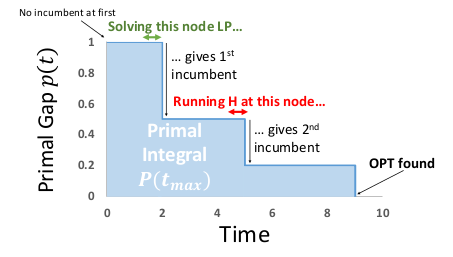
\includegraphics[width=0.7\linewidth]{primal_integral}
		\caption{Illustration de la fonction \textit{Intégrale primitive}}
		\label{fig:primalintegral}
	\end{figure}
	Au début de l'exécution, on a pas de solution, donc $p(t)$ prend la valeur 1. Au fil de l'exécution, à chaque solution trouvée, $p(t)$ se met à jour et diminue. Quand une solution optimale est trouvée, elle prend la valeur 0. L'intégrale primitive de cette fonction est la surface délimitée par $p(t)$ et les deux axes. \cite{Achterberg2012} suggèrent d'utiliser cette fonction pour mesurer l'évolution des heuristiques primitives via les solutions qu'elles trouvent à des instants $t$. Plus $P(t_{max}) $ est petit, meilleure est la solution trouvée. 
	
	Cette mesure à été testée par \cite{Achterberg2012} et par \cite{Berthold2013} sur des instances de la littérature pour mesurer l'effet des heuristiques primitives sur le processus de résolution de MIP. \cite{Berthold2013} que l'utilisation des heuristiques primitives sur ces instances améliore le résultat de 78.8 \% pour le solveur SCIP et de 86.5 \% pour IBM \textsc{Cplex}. Dans \cite{Achterberg2012}, les auteurs concluent qu'hybrider des heuristiques primitives coûteuses en temps avec d'autres pas très gourmandes en temps d'exécution donne de meilleurs résultats qu'utiliser des heuristiques coûteuses toutes seules. Ce dernier s'avère aussi meilleur qu'utiliser des heuristiques pas coûteuses en temps. Ils tirent aussi la même conclusion que précédemment, à savoir, qu'utiliser des heuristiques primitives donne de meilleure résultats que ne pas les utiliser. Cette mesure est aussi reprise dans \cite{Khalil2017} où le but est de trouver un moyen de prédire où et quand il serait intéressant de lancer une heuristique primitive dans un arbre branch and bound. Le modèle présenter fait appel à des techniques d'apprentissage (\text{Machine learning}) pour mesurer l'effet de l'appel de l'heuristique sur le un nœud donné.
	     
	%\section{Résultats des tests et comparaison entre les heuristiques primitives}
	
	% a la fin, fournir un tableau récapitulatif de tout ce qui a été dit sur les heuristiques primitives.
	
	%liste des papiers et quelques de leurs résultats généraux
	
	\section{Conclusion}
	Nous avons vu dans ce chapitre les heuristiques primitives et comment elles fonctionnent. On suivi pour cela la même classification proposée par \cite{berthold2006} à savoir les heuristiques en profondeur qui changent à chaque fois les bornes des variables jusqu'à ce qu'elle soient fixées et la plus sophistiquée d'entre elles Feasibility Pump dans ses deux versions, les heuristiques d'arrondissement qui décident d'arrondir les variables fractionnelles soit supérieurement soit inférieurement et ceci selon différents critères. Les heursitiques de propagation qui exploitent un arbre branch-and-bound auxiliaire avec des techniques de fixation et de propagation et les heuristiques d'amélioration qui commencent par une solution faisable en entrée qu'elles tentent d'améliorer. Nous avons aussi vu que pour mesurer l'impact de ces heuristiques, une fonction intégrale primitive à aussi été introduite. Elle permet de connaitre l'apport des fonctions primitives par rapport au schéma global de résolution du MIP. Selon les résultats, ces heuristiques sont prometteuses et permettent d'obtenir des solution faisable de qualité. 
	
	\chapter{Utilisation des heuristiques primitives dans la résolution de problèmes d'optimisation}
	
	\section{Introduction}
	Les heuristiques primitives sont des heuristiques venant du domaine de la programmation en nombre mixte (MIP). Elles ont donné d'assez bon résultats sur les benchmarks de la littérature des MIP \cite{berthold2006}, \cite{Achterberg2012}. \cite{Berthold2013} considère même que c'est l'un des aspects les plus importants des solveurs commerciaux de nos jours: \textit{"On the other hand, the solver vendors, such as Cplex, Gurobi or Xpress, seem to consider primal heuristics to be a "trade secret". It stays unrevealed which heuristics they use, when they are called, or just how many of them a solver features, whereas, for other components, there are plenty of user parameters and statistical outputs available. One interpretation of this discrepancy might be that primal heuristics are considered a - if not the - crucial part of the software, and their value is simply not reflected by the performance measures that we commonly use."} En effet, tous ceux qui utilisent un solveur commercial ou open-source tel que SCIP utilise d'une manière ou d'une autre les heuristiques primitives. Peu d'articles dans la littérature font mention du choix d'utilisation des heuristiques primitives dans la conception d'une solution à un problème d'optimisation. A ma connaissance, il n'y a eu aucun survey qui relate une telle utilisation pour des problèmes d'optimisation combinatoire. Ce chapitre a pour modeste but de combler un tant soit peu ce vide en recensant quelques cas d'utilisation fructueux des heuristiques primitives. Le choix des articles s'est fait sous la mention de l'heuristique utilisée donc les articles mentionnant un l'utilisation d'un solveur commercial ou open-source pour moteur de résolution de la formulation mathématique du problème ne sont pas pris en compte puisqu'il n'est pas dit quelle heuristique primitive a été utilisée. De plus, pour des mesures d'efficacités, certains on tendance à les désactiver car elles ont tendance à cacher l'effet d'autres heuristiques sur la qualité de la solution générée. Le reste du chapitre est organisé comme suit. Dans la section 2, quelques utilisation préliminaires sont répertoriées. Ce sont les premières heursitiques primitives développées. Dans la section 3, on aborde les heuristiques primitives utilisées dans les problèmes de tournées. Dans la section 4, celles utilisées dans les problèmes de réseaux sont revues.  Dans les section 5, quelques autres problèmes sont présentés avec les heuristiques primitives employées dans la résolution. Enfin, dans la section 6, un tableau récapitulatif des problèmes et des heuristiques primitives utilisées est présenté.  
	
	
	\section{Premières utilisations}
	Comme cité en introduction, les heuristiques primitives ont longtemps été présentes dans les solveurs. Par conséquent, toute implémentation les utilisant pour les problèmes d'optimisation les utilise plus ou moins involontairement et sous réserve qu'elles n'aient pas été désactivées. Néanmoins, quelques utilisations précoces peuvent être répertoriées. C'est la cas par exemple de l'heuristique primitive de Toyoda \cite{Toyoda1975}. C'est une heuristique conçue pour les problèmes en variables binaires pour lesquelles elle affecte une mesure appelée \textit{"Gradient effectif"}. Toyoda l'applique à une problème de sac à dos multidimensionnel. Les résultats des tests prouvent que la méthode est efficace pour donner des solutions approximatives avec un taux d'erreur décroissant au fur et à mesure que les instances deviennent grandes. De plus, le temps de calcul est mineur même pour de larges instances. 
	\cite{Loulou1979} s'inspire de l'heuristique de Toyoda pour le même problème et modifie l'heuristique de sélection de la prochaine variable à insérer.
	
	\cite{Holmberg} traite le problème d'emplacement d'installation. Ce problème vise à répondre à la question: Quel est le meilleur emplacement pour une installation?. Il mentionne pour cela l'utilisation d'une heuristiques nommée \textit{ADD} \cite{Domschke1985}. ADD est un algorithme glouton qui répète l'étape suivante: augmenter la taille du site $i$ qui donne la plus grande réduction du coût total. La procédure se termine quand aucune réduction n'est possible. L'algorithme ne donne pas de bons résultats, néanmoins, une amélioration de l'algorithme avec des règles de priorités existe et qui améliore quelqeu peu les résultats.

    
	\section{Heuristiques primitives dans les problèmes de tournées}
	    Les problèmes de tournées de véhicules désignent une classe de problèmes où l'on considère un ensemble de \textit{clients} et un ensemble de \textit{véhicules} situés dans un ou plusieurs \textit{dépots} répartis. Les clients, situés géographiquement à une certaines distance les uns des autres, sont reliés par un réseau de routes. Le but du problème est de déterminer un ensemble optimal de routes (chaque route sera alors appelée \textit{tournée} ) que devront parcourir les véhicules pour desservir les clients tout en minimisant une certaine quantité. Cette quantité à minimiser est généralement le nombre de véhicules à utiliser ou bien le coût de chaque tournée.
	    Les heuristiques primivites sont abordées dans les travaux de \cite{Agra2014}, \cite{Cacchiani2014} et \cite{Bettinelli2014}.
	    
	    Dans \cite{Cacchiani2014}, les auteurs présentent une méthode hybride à case d'heuristiques et de méthode exacte dans un schéma de génération de colonne. Leur algorithme consiste en une résolution par heuristique du problème maître restreint suivi d'une recherche locale. Ensuite, une procédure pour fixer les variable est exécutée. Les auteurs ont choisi de fixer définitivement les variables qui sont à 1 dans la solution partielle obtenue. Les routes qui deviennent interdites dans la solution sont ensuite propagée pour les prochaines itérations. Les résultats obtenus sont concluants et compétitifs par rapport à la littérature. De nouvelles solutions ont même été identifiées pour certaines instances du problème.
	    
	    \cite{Bettinelli2014} proposent un algorithme de branch-and-price pour la variante avec ramassage et livraison et fenêtre de temps. L'heuristique primitive introduite est un algorithme glouton assez simple. L'algorithme commence avec une route vide et sélectionne un véhicule au hasard. Les clients sont sélectionnés selon le fait qu'il augmentent le moins possible le coup total du problème. Les colonnes ainsi trouvés par l'algorithme constituent une initialisation pour le problème maître restreint dans la phase de génération de colonne. 
	    
	    \cite{Agra2014} considèrent le problème d'acheminement de stock à courte distance dans l'archipel du Cap-Vert. Ce problème traite l'acheminement et la planification des flottes de navires de pétrole entre les ports de sorte à ce que l'acheminement des produits soit satisfait sous des contraintes de temps. L'objectif est de déterminer les politiques de distribution qui minimisent les coûts de routage et d'exploitation, tout en maintenant les niveaux de stock dans leurs limites. \cite{Agra2014} utilisent une hybridation de trois heuristiques. L'heuristique \textit{Rolling horizon} considère découpe l'horizon de planification en des sous-horizons et résoud une MIP pour chaque sous-horizon. Les heuristiques primitives introduites sont \textit{Local branching} de \cite{fischetti2003local} et \textit{Feasibility Pump}  de \cite{Fischetti2005}. La première hybridation concerne \textit{Rolling Horizon} et \textit{Local Branching}. Plusieurs versions de \textit{Local branching} ont été testées, toutes diffèrent dans la manière les auteurs approchent le sous-problème. Dans la première version, la résolution du sous-problème est stoppée à la première solution trouvée. Par contre, dans la deuxième, le sous-problèmes est résolu deux fois, une première fois jusqu'à réduire un écart défini par: 
	    \begin{gather} \label{gap}
	        g = 100 \times \frac{UB-LB}{LB} \hspace{10pt}
	    \end{gather}
	    (où $UB$ est la meilleure borne supérieure et $LB$ est la meilleure borne inférieure)    
	     est réduit à 10 \% . Dans la  deuxième résolution, une contrainte défini par les auteurs est ajoutée puis l'heuristique primitive est lancée jusqu'à atteidre un écart $g$ de 5 \%. La troisième version développée ressemble à la deuxième sauf que l'on fait plus appel à la contrainte défini par les auteurs et que le critère d'arrêt est soit une limite temporelle, soit un nombre d'itération atteints sans amélioration ou bien un nombre maximal d'itération global.
	    Dans l'algorithme de \textit{Feasiblity pump}, les auteurs se sont intéressés à modifier quelques phases de l'algorithme de \cite{Fischetti2005} pour l'adapter au problème. La stratégie d'arrondissement est défini par 
	    \begin{gather}
	        x = \begin{cases}
	            1  & \text{si} \hspace{5pt} x \textgreater 0.5 \\
	            0 & \text{si} \hspace{5pt} x \textless \epsilon
	        \end{cases}
	    \end{gather}
	    Dans les tests, $\epsilon = 0.1$.
	    Ils ont introduit ensuite une fonction de distance en tenant compte des caractéristiques du problème. La perturbation introduite en cas de cycles est inspirée de celle introduite par \cite{Achterberg2007}.Dans la phase de test, \cite{Agra2014} ont fait beaucoup de combinaisons deux à deux des heuristiques et même une combinaison des trois heuristiques. Cette dernière s'est avéré être la plus fructueuse et donne les meilleurs résultats.
	  
	    
	   
	   
	   
	\section{Heuristiques primitives dans les autres problèmes d'optimisation}
	    Hors les problèmes mentionnés pour laquelle il y a eu plus de littérature, il existe certaines autres applications encore isolées pour des problèmes d'optimisation. Elles sont toutes récentes compte tenu du fait que les heuristiques primitives sont en émergence. C'est pour cela qu'il devient intéressant de constater  l'étendue de l'efficacité de ces heuristiques appliquées à ces problèmes.
	
	    \paragraph{Heuristiques primitives dans les problèmes de conception de réseaux}
	
    	   Dans le problème de conception de réseau , on se donne un réseau représenté par un graphe avec des coûts non négatifs sur les arcs. On essaie d'acheminer un ensemble $D$ de demandes via le réseau au moindre coût.\cite{buchheim2011exact} présent un algorithme de Branch-and-cut. Les heuristiques primitives utilisées dans le problèmes sont des heuristiques d'arrondissement propres aux données du problème. Les auteurs fournissent les résultats obtenus par la fonction écart $g$ telle que défini dans \ref{gap}. Dans 458 \% des cas, $g \textless 10\%$ et dans 55 \% des cas, $g \textgreater 10 \%$ avec un taux au pire des cas de $61\%$. Ce qui est un très bon score pour ces heuristiques. Les conclusions des auteurs valident leur méthode puisqu'ils arrivent à résoudre toutes les instances réalistes à optimalité.
    	
	    
	    \paragraph{Ordonnancement de l'admission des patients}
	    
	    Ce problème consiste à trouver l'affectation à un lit d'hôpital pour la durée de leur séjour se basant sur les besoins médicaux et les préférences des patients. Un modèle mathématique pour ce problèmes a été proposé par \cite{Ceschia2011}. \cite{Turhan2017} développe deux heuristiques en se servant de la formulation mathématique précédente. Il s'agit de Fix-and-relax (F\&R) et Fix-and-Optimize (F\&O). Une revue de la littérature sur l'utilisation de ces heuristiques sur d'autres problème est faite par le même auteur. Ces deux heuristiques se basent sur les MIPs avec comme principe de décomposer le problème initial en sous-problèmes. L'auteur utilise une décomposition suivant le temps et en patients. F&R génère une solution initiale qu'elle passe à F&O pour l'améliorer.
	    Les heuristiques ont été testé sur les benchmark de Demeester (https://people.cs.kuleuven.be/~wim.vancroonenburg/pas/). Les tests ont révélé que la fonction objectif a un écart de 5 à 15 pourcent des la meilleure solution connue en un temps raisonnable.  
	    
	    \paragraph{Le problème des (r|p)-centroïdes discrets}
	    
	    Ce problème modélise un leader et son concurrent qui sont en compétition pour attirer des clients vers leur marché et maximiser les gains. Au début, le leader ouvre $p$ installations et le concurrent $r$ installation. \cite{Alekseeva2010} mentionne que c'est un jeu de Stackelberg non-coopératif. L'auteur donne la formulation mathématique du problème et propose une méthode exacte itérative au problème. L'une des étapes de cet algorithme cherche la solution optimale d'un problème défini par un sous-ensemble de contraintes. Cette partie étant très coûteuse en temps, Alekseeva et al. la remplacent par un autre problème de faisabilité plus facile à résoudre et ne nécessitant pas une preuve d'optimalité. Pour le résoudre \cite{Alekseeva2010} propose d'utiliser Feasibility pump de \cite{Fischetti2005}. Les résultats de l'auteur ne sont pas vraiment concluent puisque les concurrent obtient plus de 50\% du marché dans tous les benchmarks. Néanmoins, le problème de faisabilité à été résolu avec succès à chaque itération avec feasibility pump.
	    
	    \paragraph{Le problème d'emplacement de hub}
            
            Selon \cite{Alumur2008}, ce problème se concentre sur la localisation des installations de hub et l'allocation de noeuds clients (trafic réseau) vers le hub et depuis le hub vers le destinataire.  Deux type de réseau de hub existent: a) avec allocation unique où tous les signaux allant et venant d'un centre passent par un seul hub. b) avec multiple allocation où chaque centre peut envoyer et recevoir des signaux à partir de plusieurs hub. La littérature sur le sujet assume trois suppositions sur le problème:
            \begin{enumerate}
                \item Le réseau du hub est complet (i.e. il y a un lien entre chaque pair de hub);
                \item Il y a des économies à réaliser à faire des connexions inter-hub;
                \item Aucun service direct entre les centre n'est permis.
            \end{enumerate}
            
            \cite{He2015} propose une heuristique nommée IMMIP \textit{(IMproved MIP)} se basant sur le branch-and-bound, la relaxation lagrangienne et la programmation linéaire. Il décrit cette heuristique comme étant similaire certaines heursitiques primitives dont feasibility pump, \textsc{Rins}, \textsc{Rens} et relax-and-fix. Par conséquent, même si ce n'est pas explicitement mentionné dans l'article, on peut supposer que c'est aussi une heuristique primitive.
          
            Selon \cite{He2015}, l'heuristique IMMIP génère une solution initiale faisable et une solution relaxée du MIP (la LP-relaxation) et après utilise ces solutions pour construire une fonction de probabilité qui va fixer les variables entières.
          
            L'auteur offre aussi une étude théorique comparative entre l'heuristique IMMIP et les autres heuristiques primitives dont il s'inspire. IMMIP est similaire aux heuristiques primitives dans le fait qu'elles créent toutes un sous-MIP où une partie des variables entières est fixé puis ce sous-MIP est résolu pour obtenir une solution faisable au MIP originel. La différence entre cette heuristique et les heuristiques primitives est la façon dont les solutions sont utilisées pour construire les sous-MIP.      
            
            Les résultats des tests montrent que l'heuristique IMMIP offre des solution de qualité supérieure à celles des autres heuristiques primitives avec des écarts avec la solution optimale plus stables que celui des autres méthodes. He et al. envisagent même d'étendre la méthode à d'autres problèmes ayant une formulation en MIP.
            
	    \paragraph{Problème du voyageur du commerce}
	    
	        Plus précisément, il s'agit du problème du voyageur du commerce avec dépendances temporelle qui est traité dans \cite{hansknecht2018cuts}. Cette variante généralise le problème du voyageur du commerce, en plus de prendre en considération le coût d'un voyage entre deux ville, celui-ci change à travers le temps. Ce qui rend le problème plus difficile que le problème du voyageur du commerce. \cite{hansknecht2018cuts} propose deux formulations, l'une basée sur les arcs et l'autre basée sur les chemins. Puis, ils font l'étude de la structure  du problème et mettent en évidence certaines inégalités valides. Ils proposent ensuite, pour chaque formulation un algorithme de branch-and-bound. Les auteurs ont mis des efforts sur l'étude du problème et sur les heuristiques primitives. Les heuristiques primitives utilisées sont celle de branchement et celles de propagation. Ils se sont servis de celles se trouvants dans le solveur SCIP. Selon les résultats de leurs tests, les heuristiques primitives réduisent considérablement l'écart restant après l'ajout des inégalités.
	    
	    
	    \paragraph{Problème d'affectation généralisé}
	        Dans \cite{sadykov2018primal}, les auteurs présentent des heuristiques en profondeur adaptées pour le cas de la génération de colonne. Ces méthodes sont intégrées ensuite dans un branch-and-price. Le but étant de créer des méthodes génériques pour le branch-and-price, leurs travaux se basent sur les heuristiques primitives de \cite{fischetti2003local}, \cite{Fischetti2005}, \cite{danna2005exploring} et \cite{berthold2006}.
	        Ils présentent cinq variantes des heuristiques en profondeur: \textit{pure diving, diving with limited backtrack, strong diving, diving with restarts, diving with sub-MIPing}, ainsi qu'une heuristique de branchement local et une adapatation de feasibiliry pump au cas de la génération de colonne. Les tests on été effectués sur le problème d'affectation généralisé. Pour rappel, dans ce problème, on a $n$ tâches qu'on veut affecter à $m$ machines. Chaque machine $i$ a une capacité $u_i$ et chaque tâche $j$ assigné à une machine $i$ utilise $d_{ij}$ ressources et coûte $c_{ij}$. Le but est d'affecter une tâche à exactement une machine de telle sorte que les total des ressources consommées par chaque machine ne dépasse pas sa capacité. Un test sur des benchmarks de la littérature issues de http://www.al.cm.is.nagoya-u.ac.jp/~yagiura/gap/ montrent que \textit{pure diving} est l'heuristique la plus rapide mais la qualité de la solution n'est pas bonne avec un pourcentage de 0\% de solutions optimales trouvées et de 70\% de solutions faisables trouvées. La meilleure étant \textit{strong diving} avec une pourcentage de 15\% de solutions optimales trouvées et 100\% de solutions faisables mais un temps d'exécution relativement plus lent (30 fois plus lente que \textit{pure diving}). Les auteurs concluent aussi que le meilleur compromis entre les deux est l'algorithme de \textit{diving with limited backtracking}, 5 fois plus lente que \textit{pure diving} mais avec 100\% de solutions faisables trouvées dont 5\% sont optimales. Une comparaison avec les résultats de \cite{Yagiura2006} montrent aussi que l'algorithme \textit{diving with limited backtracking} montrent aussi que l'algorithme est en moyenne plus rapide et donne de meilleurs résultats. Les auteurs rapportent aussi une amélioration de la meilleure solution de 10 instances de la littérature dont deux instances pour lesquelles elle trouve une solution optimale pour la première fois. 
	        
	    \paragraph{Problème de coloration de graphes}
	        \cite{sadykov2018primal} continuent le tests des mêmes heuristiques citées pour le problème d'affectation généralisée avec le problème de coloration de graphes. L'objectif étant d'affecter aux noeuds d'un graphe une couleur de façon à ce que deux noeuds adjacents n'aient pas la même. On cherche minimiser le nombre de couleurs employées pour un graphe donné.
	        Les instances utilisées sont générées au hasard pour un nombre variable de noeud dans le graphe entre 50 et 90 avec un pas de 10. Au total 125 instances ont été générées. Comme pour le problème d'affectation généralisé, \textit{pure diving} est la plus rapide mais le nombre de solutions optimales n'est que de 71\%. Ce nombre est bien inférieur par rapport à \textit{strong diving} qui donne 94\% de solutions optimales mais contre un temps d'exécution plus grand (presque 4 fois plus long que \textit{pure diving}). L'heuristique \textit{diving with limited backtracking} se situe toujours comme un compromis entre les deux avec un temps d'exécution de 1.46 fois plus long que \textit{pure diving} et 88\% de solutions optimales. En comparaison avec les méthodes de la littérature Sadykov et al. trouvent des résultats éloignés en moyenne d'une unité par rapport aux résultats optimaux. De plus, l'heuristique est plus performantes que certaines heursitiques récentes. 
	    
	    \paragraph{ les problèmes de bin packing}
	       Dans le problème de bin packing, on a $n$ objets qu'on désire placer dans des boites de taille $T$. Chaque objet $i$ a $d_i$ copies de taille $t_i$. Le problème consiste à minimiser le nombre de boîtes nécessaires pour qu'à la fin, chaque objet puisse être placé dans une boîte de telle sorte que la taille total des toutes les copies assignées à une boîte ne dépasse pas $T$. Sadykov et al. traitent ce problème comme troisième exemple d'application des heuristiques en profondeur dans \cite{sadykov2018primal}. Les résultats suivent le même schéma que pour les autres problèmes. \textit{Pure diving} se distingue par sa vitesse mais néanmoins des résultats moins bons que ceux de \textit{strong diving} qui semble confirmer être la meilleure mais aussi la plus coûteuse en temps d'exécution. \textit{Diving with limited backtracking} se classe toujours en meilleur rapport temps d'éxécution/qualité des résultats avec des résultats très proches de ceux de \textit{strong diving} sur toutes les instances.
	\section{Récapitulatif}
	Le tableau suivant résume tous les problèmes vus dans les sections précédentes. Pour chaque problème, les heuristiques primitives employées sont mentionnées.
	    \begin{center}
                \begin{tabularx}{1\textwidth}{|X|X|X|X|}
                    \hline
                    Article & Problème & Heuristique(s) primitive(s) employée(s) & Année\\ 
                    \hline
                    \hline
                    \cite{Toyoda1975} & Sac à dos multidimensionnel & Gradient effectif & 1975\\  \hline
                    \cite{Turhan2017}& Ordonnancement de l'admission des patients & Fix-and-relax & 2017 \\
                    && Fix-and-optimize & 2017\\ \hline 
                    \cite{Alekseeva2010} & (r|p)-centroïdes discrets & Feasibility pump & 2010\\ \hline 
                    \cite{He2015} & Le problème d'emplacement de hub & IMMIP & 2015 \\ \hline
                    \cite{hansknecht2018cuts} & Problème du voyageur du commerce & Heuristiques de branchement et de propagation de SCIP & 2018  \\ \hline
                    \cite{sadykov2018primal} & Problème d'affectation généralisé & Heuristiques en profondeur ( Pure diving, Diving with limited backtracking, Strong diving, Didiving with restarts, diving with sub-MIPing) & 2018\\
                    &Problème de coloration de graphe& heuristique de branchement local & 2018\\
                    &Problème de bin packing& feasibiliry pump & 2018 \\ \hline
                     \cite{Cacchiani2014} & Problème de tournée de véhicule & Heuristique de fixation & 2014 \\ \hline
                     \cite{Bettinelli2014}& Problème de tournée de véhicule & Algorithme glouton & 2014 \\ \hline
                     \cite{Agra2014} & Problème d'acheminement de stock à courte & \textit{Feasibility pump} & 2014 \\
                     & &  \textit{Local branching} & \\ \hline
                     \cite{buchheim2011exact} & Le problème de conception de réseau & \textit{Heuristiques d'arrondissement} & 2011 \\ \hline
                    
            \end{tabularx}    
        \end{center}
        
    
	\section{Conclusion}
	On a vu dans les sections précédentes quelques applications des heuristiques primitives sur des problèmes d'optimisation. Ces applications sont plutôt fructueuses dans la plupart des problèmes mentionnés voire même meilleures que certaines méthodes de la littérature. La plupart des applications mentionnées sont récentes ce qui tant à montrer l'émergence des heuristiques primitives dans le domaine et le vif intérêt qu'elles commencent à susciter. Pour finir, un tableau récapitulatif résume les problèmes abordés ainsi que les heuristiques primitives employés pour résoudre. 
	La variété des problèmes traités par ces heuristiques leur permet d'être essayée sur des instances plus concrètes et donc plus difficiles que les instances dédiées aux MIPs qui n'imposent pas d'interprétation des résultats. Cela est est un point positif qui permettra des les améliorer et de toucher plus d'application qu'elles n'en traitent déjà.
	
	
	\chapter*{Conclusion}
	A travers ce travail, nous nous sommes intéressés aux méthodes exactes pour la résolution de problèmes d'optimisation. Plus particulièrement, nous avons vu les méthodes arborescentes. A travers le premier chapitre, une revue du branch-and-bound et de ses variantes à été effectué. On a pu voir les principaux choix qui s'imposent de faire pour chaque étape du branch-and-bound, que ce soit pour le choix de départ, la phase de branchement, les méthodes de parcours ou bien le calcul des bornes. Ce sont les principaux critères qui influencent le succès d'une méthode branch-and-bound. Les variantes qui ont le plus de succès sont le branch-and-cut qui incorpore les coupes planes et le branch-and-price qui lui utilise la méthode de génération de colonnes. Quelques applications fructueuses des méthodes arborescentes pour la résolution de problèmes d'optimisation ont aussi été évoquées. Une application majeure du branch-and-bound sont les MIPs. C'est pour cela que dans le chapitre deux, on a fait une revue des heuristiques simulant un arbre branch-and-bound et donnant une solution faisable de bonne qualité pour les MIP. Ce sont les heuristiques primitives. Enfin, dans le dernier chapitre, on a pu voir quelques applications des heuristiques primitives pour la résolution de problèmes d'optimisation. Ces applications montrent que les heuristiques primitives peuvent se montrer puissantes et donner des résultats concurrençant des méthodes de la littérature des problèmes étudiés. Aussi, cela montre l'importance de pouvoir modéliser un problème sous forme de MIP pour pouvoir bénéficier d'un large éventail de méthode de traitement. 
	
	Dans les futurs travaux, on peut étudier les heuristiques primitives dans le cas de programmes quadratiques ou non-linéaires en générales. Ils constituent une classe de problèmes plus difficiles que les MIPs. Des travaux dans ce sens ont été initié par \cite{Berthold2014} mais peuvent encore être étendu par de nouvelles méthodes. L'application de ces heuristiques aux problèmes d'optimisation serait aussi un point intéressant à aborder. Cela permettra de tester ces heuristiques sur des problèmes moins abstraits que ceux des benchmarks de la littérature.
	
	\newpage
	\bibliographystyle{apacite}
	\bibliography{references_pfe.bib} 
	

\end{document}